% Options for packages loaded elsewhere
\PassOptionsToPackage{unicode}{hyperref}
\PassOptionsToPackage{hyphens}{url}
\PassOptionsToPackage{dvipsnames,svgnames,x11names}{xcolor}
%
\documentclass[
]{agujournal2019}

\usepackage{amsmath,amssymb}
\usepackage{iftex}
\ifPDFTeX
  \usepackage[T1]{fontenc}
  \usepackage[utf8]{inputenc}
  \usepackage{textcomp} % provide euro and other symbols
\else % if luatex or xetex
  \usepackage{unicode-math}
  \defaultfontfeatures{Scale=MatchLowercase}
  \defaultfontfeatures[\rmfamily]{Ligatures=TeX,Scale=1}
\fi
\usepackage{lmodern}
\ifPDFTeX\else  
    % xetex/luatex font selection
\fi
% Use upquote if available, for straight quotes in verbatim environments
\IfFileExists{upquote.sty}{\usepackage{upquote}}{}
\IfFileExists{microtype.sty}{% use microtype if available
  \usepackage[]{microtype}
  \UseMicrotypeSet[protrusion]{basicmath} % disable protrusion for tt fonts
}{}
\makeatletter
\@ifundefined{KOMAClassName}{% if non-KOMA class
  \IfFileExists{parskip.sty}{%
    \usepackage{parskip}
  }{% else
    \setlength{\parindent}{0pt}
    \setlength{\parskip}{6pt plus 2pt minus 1pt}}
}{% if KOMA class
  \KOMAoptions{parskip=half}}
\makeatother
\usepackage{xcolor}
\setlength{\emergencystretch}{3em} % prevent overfull lines
\setcounter{secnumdepth}{5}
% Make \paragraph and \subparagraph free-standing
\makeatletter
\ifx\paragraph\undefined\else
  \let\oldparagraph\paragraph
  \renewcommand{\paragraph}{
    \@ifstar
      \xxxParagraphStar
      \xxxParagraphNoStar
  }
  \newcommand{\xxxParagraphStar}[1]{\oldparagraph*{#1}\mbox{}}
  \newcommand{\xxxParagraphNoStar}[1]{\oldparagraph{#1}\mbox{}}
\fi
\ifx\subparagraph\undefined\else
  \let\oldsubparagraph\subparagraph
  \renewcommand{\subparagraph}{
    \@ifstar
      \xxxSubParagraphStar
      \xxxSubParagraphNoStar
  }
  \newcommand{\xxxSubParagraphStar}[1]{\oldsubparagraph*{#1}\mbox{}}
  \newcommand{\xxxSubParagraphNoStar}[1]{\oldsubparagraph{#1}\mbox{}}
\fi
\makeatother


\providecommand{\tightlist}{%
  \setlength{\itemsep}{0pt}\setlength{\parskip}{0pt}}\usepackage{longtable,booktabs,array}
\usepackage{calc} % for calculating minipage widths
% Correct order of tables after \paragraph or \subparagraph
\usepackage{etoolbox}
\makeatletter
\patchcmd\longtable{\par}{\if@noskipsec\mbox{}\fi\par}{}{}
\makeatother
% Allow footnotes in longtable head/foot
\IfFileExists{footnotehyper.sty}{\usepackage{footnotehyper}}{\usepackage{footnote}}
\makesavenoteenv{longtable}
\usepackage{graphicx}
\makeatletter
\newsavebox\pandoc@box
\newcommand*\pandocbounded[1]{% scales image to fit in text height/width
  \sbox\pandoc@box{#1}%
  \Gscale@div\@tempa{\textheight}{\dimexpr\ht\pandoc@box+\dp\pandoc@box\relax}%
  \Gscale@div\@tempb{\linewidth}{\wd\pandoc@box}%
  \ifdim\@tempb\p@<\@tempa\p@\let\@tempa\@tempb\fi% select the smaller of both
  \ifdim\@tempa\p@<\p@\scalebox{\@tempa}{\usebox\pandoc@box}%
  \else\usebox{\pandoc@box}%
  \fi%
}
% Set default figure placement to htbp
\def\fps@figure{htbp}
\makeatother
% definitions for citeproc citations
\NewDocumentCommand\citeproctext{}{}
\NewDocumentCommand\citeproc{mm}{%
  \begingroup\def\citeproctext{#2}\cite{#1}\endgroup}
\makeatletter
 % allow citations to break across lines
 \let\@cite@ofmt\@firstofone
 % avoid brackets around text for \cite:
 \def\@biblabel#1{}
 \def\@cite#1#2{{#1\if@tempswa , #2\fi}}
\makeatother
\newlength{\cslhangindent}
\setlength{\cslhangindent}{1.5em}
\newlength{\csllabelwidth}
\setlength{\csllabelwidth}{3em}
\newenvironment{CSLReferences}[2] % #1 hanging-indent, #2 entry-spacing
 {\begin{list}{}{%
  \setlength{\itemindent}{0pt}
  \setlength{\leftmargin}{0pt}
  \setlength{\parsep}{0pt}
  % turn on hanging indent if param 1 is 1
  \ifodd #1
   \setlength{\leftmargin}{\cslhangindent}
   \setlength{\itemindent}{-1\cslhangindent}
  \fi
  % set entry spacing
  \setlength{\itemsep}{#2\baselineskip}}}
 {\end{list}}
\usepackage{calc}
\newcommand{\CSLBlock}[1]{\hfill\break\parbox[t]{\linewidth}{\strut\ignorespaces#1\strut}}
\newcommand{\CSLLeftMargin}[1]{\parbox[t]{\csllabelwidth}{\strut#1\strut}}
\newcommand{\CSLRightInline}[1]{\parbox[t]{\linewidth - \csllabelwidth}{\strut#1\strut}}
\newcommand{\CSLIndent}[1]{\hspace{\cslhangindent}#1}

\usepackage{fontspec}
\usepackage{multirow}
\usepackage{multicol}
\usepackage{colortbl}
\usepackage{hhline}
\newlength\Oldarrayrulewidth
\newlength\Oldtabcolsep
\usepackage{longtable}
\usepackage{array}
\usepackage{hyperref}
\usepackage{float}
\usepackage{wrapfig}
\usepackage{url} %this package should fix any errors with URLs in refs.
\usepackage{lineno}
\usepackage[inline]{trackchanges} %for better track changes. finalnew option will compile document with changes incorporated.
\usepackage{soul}
\linenumbers
\makeatletter
\@ifpackageloaded{caption}{}{\usepackage{caption}}
\AtBeginDocument{%
\ifdefined\contentsname
  \renewcommand*\contentsname{Table of contents}
\else
  \newcommand\contentsname{Table of contents}
\fi
\ifdefined\listfigurename
  \renewcommand*\listfigurename{List of Figures}
\else
  \newcommand\listfigurename{List of Figures}
\fi
\ifdefined\listtablename
  \renewcommand*\listtablename{List of Tables}
\else
  \newcommand\listtablename{List of Tables}
\fi
\ifdefined\figurename
  \renewcommand*\figurename{Figure}
\else
  \newcommand\figurename{Figure}
\fi
\ifdefined\tablename
  \renewcommand*\tablename{Table}
\else
  \newcommand\tablename{Table}
\fi
}
\@ifpackageloaded{float}{}{\usepackage{float}}
\floatstyle{ruled}
\@ifundefined{c@chapter}{\newfloat{codelisting}{h}{lop}}{\newfloat{codelisting}{h}{lop}[chapter]}
\floatname{codelisting}{Listing}
\newcommand*\listoflistings{\listof{codelisting}{List of Listings}}
\makeatother
\makeatletter
\makeatother
\makeatletter
\@ifpackageloaded{caption}{}{\usepackage{caption}}
\@ifpackageloaded{subcaption}{}{\usepackage{subcaption}}
\makeatother

\usepackage{bookmark}

\IfFileExists{xurl.sty}{\usepackage{xurl}}{} % add URL line breaks if available
\urlstyle{same} % disable monospaced font for URLs
\hypersetup{
  pdftitle={AqC 6.3},
  pdfauthor={Valdrich Fernandes; Perry de Louw; Coen Ritsema; Ruud Bartholomeus},
  colorlinks=true,
  linkcolor={blue},
  filecolor={Maroon},
  citecolor={Blue},
  urlcolor={Blue},
  pdfcreator={LaTeX via pandoc}}


\journalname{Water Resource Research}

\draftfalse

\begin{document}
\title{AqC 6.3}

\authors{Valdrich Fernandes\affil{1}, Perry de Louw\affil{1,2}, Coen
Ritsema\affil{1}, Ruud Bartholomeus\affil{1,3}}
\affiliation{1}{Soil Physics and Land Management group, Wageningen
University \& Research, Wageningen, the
Netherlands}\affiliation{2}{Department of Soil and
Groundwater, Deltares, Utrecht, the Netherlands}\affiliation{3}{KWR
Water Research Institute, Nieuwegein, the Netherlands}
\correspondingauthor{Valdrich Fernandes}{valdrich.fernandes@wur.nl}


\begin{abstract}
Managed Aquifer Recharge (MAR) is widely applied to enhance groundwater
storage and promote the sustainable use of this essential resource.
Techniques such as Machine Learning (ML) as surrogate for
computationally intensive numerical models, are increasingly considered
for identifying suitable locations for MAR. While ML has been
demonstrated to be suitable for steady-state simulations, its
application for transient modelling is much more challenging. However,
understanding how water recharged during wet periods is retained and
remains available during dry periods is critical, highlighting the
importance of transient responses. In this study, we therefore employed
ML to mimic the transient effect of MAR by decomposing the time series
of groundwater storage when MAR stopped into two components---the
MAR-response and the decay coefficient---based on the observation that
the storage decays following an exponential curve. This decomposition
provides a simplified yet effective representation of groundwater
storage changes over time. Using U-Net and XGBoost, we demonstrated that
ML can accurately capture these dynamics for the Baakse Beek catchment,
located in the drought sensitive sandy soils of the Netherlands. The ML
models achieved an R\textsuperscript{2} of more than 0.85 in predicting
the two components of the long-term dynamics of the stored water.
Additionally, using explainable AI techniques, specifically SHapley
Aditive exPlanation values, we identified the site management decisions
and the properties of the surface water network near the recharge site
most significantly impact the effectiveness of the MAR in the region.
This focus on model interpretability ensures transparency in the
predictions, improving on the models' generalizability and fosters trust
among hydrologists and stakeholders.
\end{abstract}





\section{Introduction}\label{introduction}

Seasonal water availability has increasingly become a concern worldwide.
Even countries with typically robust water systems have recently faced
periods of water stress during extended periods of droughts. The
2018-2020 drought, for instance, affected most of continental Europe,
limiting surface water availability in major international rivers
(Rakovec et al., 2022). Similar extended periods of droughts are
expected to become more frequent in future climatic conditions (Aalbers
et al., 2023; Gu et al., 2023; Hari et al., 2020; van der Wiel et al.,
2021). The 2018 drought saw a general deterioration of surface water
quality, further exacerbating the stress on water users dependent on
these sources (Wolff \& van Vliet, 2021). This combination of poor water
quality and scarcity is expected to worsen in Western Europe,
particularly between June and October (Jones et al., 2024). Capturing
excess water during the seasonal surplus could help mitigate some of the
demand during the dry season.

Addressing this vulnerability requires prioritizing water management
solutions that increase summer water availability (Bartholomeus et al.,
2023), while still accounting for risks of floods and waterlogging.
Efficient groundwater management could address some of the vulnerability
by serving as a buffer, capturing water during surplus that supports
demands during dryer periods. While much of this recharge occurs
naturally, it can be further enhanced by recharging surplus water into
the groundwater aquifers using Managed Aquifer Recharge (MAR) techniques
(Dillon et al., 2019, 2020; Hartog \& Stuyfzand, 2017).

In a previous study, we demonstrated U-Net's potential to estimate the
steady-state groundwater response to MAR (Fernandes et al., 2024)
through a technique called surrogate modelling. The surrogate model is a
computationally simplified model trained on data generated using the
computationally expensive model. However, the steady-state MAR response
typically does not describe the transient behaviour of MAR, as water is
recharged during periods with a water surplus, to buffer the water
availability using the subsurface. The first goal of this paper
therefore is to investigate a potential technique for ML to capture the
transient dynamics of groundwater response to MAR capturing both
immediate effects and longer-term dynamics during periods without
recharge.

In addition to capturing the transient behaviour of MAR systems in ML,
we focus on model interpretability. Dai et al. (2024) identified
interpreting the ML models to be complex and cumbersome. However, we
hypothesize that by using explainable AI techniques such as SHapley
Aditive exPlanation (SHAP) on ML models, the relations identified by the
ML model can be explained, further building trust in the ML model.

SHAP is a powerful model interpretation technique that quantifies the
contribution of each input feature to a model's predictions, offering
detailed insights into the relations identified by the model. By
quantifying the contribution of each feature, SHAP not only indicates
the importance but also the direction of the effect of that feature on
the model's prediction. Furthermore, by evaluating feature contributions
across an entire dataset, SHAP uncovers the generalized relations that
underpin the model's predictions, unlike traditional local sensitivity
analysis that focuses on features at an individual observation. This
dataset-wide perspective allows for identifying consistent, generalized
effects of the inputs on the outputs, which could serve as a foundation
for other Multi-Critera Decision Analysis (MCDA).

In this study, we thus present ML surrogate models to efficiently and
accurately predict the transient dynamics of groundwater response to
MAR, capturing the recharging process of MAR during periods of water
surplus and the decay or discharge of the stored water volume during
periods without recharge. By calculating the SHAP values of the
surrogate model, we identify and quantify the influence of each
geo-hydrological input on the groundwater response, providing
explainable insights into the model's prediction. These insights not
only enhance our understanding of the system but also lay the groundwork
for integrating MCDA to identify potential locations for MAR. Through
this approach, we aim to develop a comprehensive understanding of the
key criteria influencing water storage due to MAR in the short to
medium-term period.

\section{Methodology}\label{methodology}

\subsection{General overview}\label{general-overview}

The methodology employed in this study borrows from Fernandes et al.
(2024), where the groundwater response to hypothetical MAR sites are
simulated with a numerical groundwater model, which makes up the
training and testing data for the ML surrogate models. The groundwater
response is calculated as the difference in the groundwater heads
between scenarios with MAR and a scenario with only natural recharge.
The location, size, and recharge rate are selected randomly to represent
the entire range of possibilities within the demonstration region. As a
continuation from Fernandes et al. (2024), we demonstrate the
applicability of the surrogate modelling technique for the Baakse Beek
catchment, which is located in the eastern sandy soils of the
Netherlands. This region is characterised by highly transmissive and
freely draining soils with a dense surface water network of ditches and
streams that drain the groundwater reservoir. This network has been
significantly intensified over time, increasing the region's
vulnerability to water shortages during extended dry periods. In this
study, we study how the water recharged by MAR decays to the natural
groundwater levels during dry periods, periods without MAR.

\subsection{Groundwater models}\label{groundwater-models}

The artificial recharge is simulated using a groundwater model, AMIGO
(Vreugdenhil, 2021), which represents the subsurface in the part of
Gelderland province that is under the jurisdiction of the water board
Rijn en IJssel in the Netherlands. AMIGO is a coupled
unsaturated-saturated zone model similar to those used in Querner et al.
(2016), and van Walsum \& Veldhuizen (2011) where the saturated zone is
represented using MODFLOW-2005 (Harbaugh, 2005) while the unsaturated
zone is represented using MetaSWAP. Gridded meteorological data from the
AMIGO dataset, including precipitation and Makkink reference crop
evaporation, is applied with the MetaSWAP that calculates the effective
groundwater recharge, which is then applied to the saturated zone model.
The saturated zone represents a 200 m thick sequence of Pleistocene
sands, which is underlain by the clayey Breda formation. This formation
represents the model basement, represented in the model by a no-flow
boundary condition. Further details of the meteorological conditions and
the model are available in Vreugdenhil (2021) and Fernandes et al.
(2024). The model extent and the boundary conditions used to represent
the Baakse Beek catchment were the same as in Fernandes et al. (2024),
except for the outer boundary conditions and the river levels for the
IJssel River to the west, where temporal data was available. The
time-varying groundwater heads at the outer boundary were derived from a
long-term simulation that is detailed in Vreugdenhil (2021). The initial
groundwater head is also derived from this long-term simulation and is
detailed in Section~\ref{sec-scenarios-considered}. Furthermore, monthly
river stage data is used for the IJssel River to the east.

In the simulated scenarios, the artificial recharge is simulated using
the Recharge (RCH) package in MODFLOW as in Fernandes et al. (2024).
This recharge is applied directly to the saturated zone, bypassing the
unsaturated zone. It represents the effective recharge rate that reaches
the saturated zone and is analogous to aquifer recharge applied below
the surface, such as through sub-surface irrigation. As a result, the
recharged water does not influence the evapotranspiration, except due to
the increase in the groundwater level. While this is a simplification of
reality, this assumption has minimum impact on the system, especially
away from the recharge site. At the recharge site, we underestimate the
evaporation and consequently overestimate the effective recharge site.

\subsection{MAR Scenarios}\label{sec-scenarios-considered}

In the scenarios considered, MAR is only applied in months when
precipitation exceeds the evaporation demand for a year with average
meteorological conditions. For this analysis, the meteorological data
from the Hupsel station, data made available by the Royal Netherlands
Meteorological Institute (KNMI), is analyzed as it is located within the
study area. Complete data is available from October 1993 onwards based
on which the annual cumulative evaporation excess precipitation is
calculated. Based on the 31 years of available data, 2012 was selected
as a representative year for average meteorological conditions, thas the
precipitation excess fell within the 25th to 75th percentile for most of
the year (see Figure~\ref{fig-precip}). The cumulative precipitation
surplus at Hupsel increased between October 1, 2011, and March 1, 2012
(blue shaded region in Figure~\ref{fig-precip}), indicating higher water
availability for artificial recharge. In the scenarios considered,
artificial recharge was simulated during this period of water surplus
and the progression of the groundwater response during the period
without artificial recharge was analyzed until October 1, 2012.

To ensure representative antecedent conditions for all scenarios, a
two-year start-up run was simulated from 1st October 2009 to 30th
September 2011. The initial groundwater levels for this start-up run
were derived from a simulation starting in April 2004, which was
conducted outside the scope of this study. Since initial soil moisture
conditions for MetaSWAP were unavailable for this earlier run,
conditions that would ensure an average recharge flux were used as the
starting conditions for the start-up run.

We simulated a total of 720 artificial recharge sites, evenly spaced
across the model domain. The recharge rate at these sites ranged from 5
to 25 mm/day, and the site sizes varied between 0.1 and 1 km². The
recharge rate and the size of each site were selected randomly using a
Latin hypercube sampling technique, similar to the methodology employed
by Fernandes et al. (2024). Six recharge sites were simulated
simultaneously in each scenario to reduce the number of groundwater
model simulations needed. The interaction between the recharge sites was
minimized by maintaining a separation distance of six times the leakage
factor between the sites. This distance ensures that groundwater levels
return to their natural state between adjacent recharge sites, hence
minimizing the interaction between the sites.

\begin{figure}

\centering{

\pandocbounded{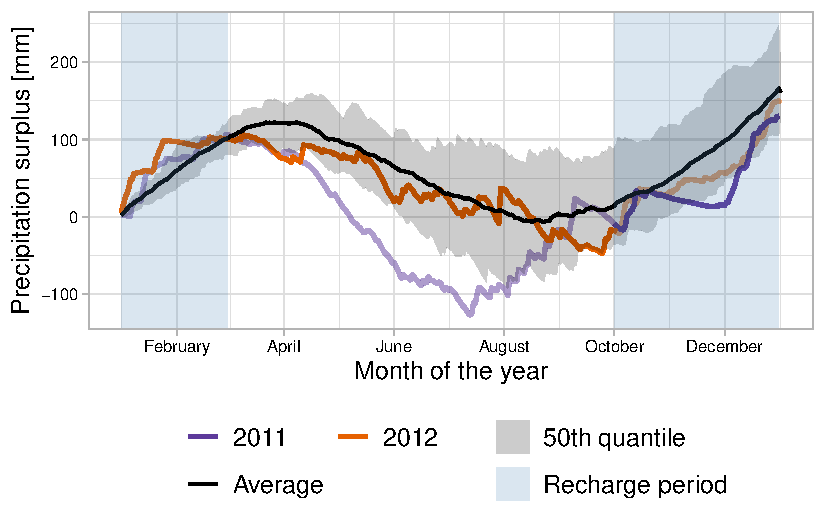
\includegraphics[keepaspectratio]{AqC6.3_paper2_V4_files/figure-pdf/fig-precip-1.pdf}}

}

\caption{\label{fig-precip}Cumulative potential precipitation surplus
(i.e.~precipitation minus reference evaporation according to Makkink
(1957)) in the simulated years, 2011 and 2012 as compared to the average
surplus between 1993 and 2024. Artificial recharge is applied between
1\textsuperscript{st} October 2011 till 1\textsuperscript{st} March
2012, when precipitation exceeds the reference evaporation.}

\end{figure}%

\subsection{Progression of the storage during the summer
season}\label{progression-of-the-storage-during-the-summer-season}

In this study, we aim to predict the progression of groundwater storage
during periods without MAR. Groundwater storage is defined as the total
increase in groundwater heads, analogous to the volume of the aquifer
saturated due to MAR. Rather than predicting the complete time series of
the groundwater storage in the period without MAR, we decompose it into
two parameters of the exponential decay function. The response peaks
during the recharge period and then gradually returns to natural
groundwater levels once recharge stops. Simulation results (see
Figure~\ref{fig-response_ts}) suggest that this decay follows an
exponential curve, a pattern commonly observed in systems where the rate
of change is proportional to the current quantity. This behaviour is
also found in the discharge from a linear reservoir in hydrology, which
decays exponentially after precipitation ends. In such reservoirs, the
discharge \(Q_t\) at time \(t\) is directly proportional to the water
storage \(S_t\) within the catchment, governed by the reservoir constant
\(k\) (Dingman, 2015; Pedersen et al., 1980; Wittenberg, 1994). This
relationship is captured in Equation~\ref{eq-linear-reservoir1}, with
the change in discharge over time described by
Equation~\ref{eq-linear-reservoir-dq}. Assuming no external fluxes like
recharge or extraction, the storage dynamics can be derived as shown in
Equation~\ref{eq-linear-reservoir-dqS}.

In this analogy, the groundwater response to artificial recharge can be
compared to the storage \(S\) in a linear reservoir. The initial storage
\(S_0\) represents the MAR-response, or the groundwater response at the
end of the recharge period, while the reservoir constant \(k\) serves as
the decay coefficientwhich defines the rate at which the groundwater
storage is drained to the surface water network. By estimating these two
parameters, the progression of groundwater storage after the recharge
period can be effectively described, providing a clear understanding of
how the system returns to equilibrium. These two parameters, the
MAR-response and the decay coefficient, are the target variables for the
ML models. These terms are used throughout the paper to identify the two
separate phases of MAR.

\begin{equation}\phantomsection\label{eq-linear-reservoir1}{
Q_t = k \cdot S_t
}\end{equation}

\begin{equation}\phantomsection\label{eq-linear-reservoir-dq}{
Q_t = Q_0 \cdot e^{-k \times t}
}\end{equation}

\begin{equation}\phantomsection\label{eq-linear-reservoir-dqS}{
S_t = S_0 \cdot e^{-k \times t}
}\end{equation}

\subsection{ML procedure}\label{ml-procedure}

\global\setlength{\Oldarrayrulewidth}{\arrayrulewidth}

\global\setlength{\Oldtabcolsep}{\tabcolsep}

\setlength{\tabcolsep}{2pt}

\renewcommand*{\arraystretch}{1.5}



\providecommand{\ascline}[3]{\noalign{\global\arrayrulewidth #1}\arrayrulecolor[HTML]{#2}\cline{#3}}

\begin{longtable}[c]{|p{1.92in}|p{3.03in}|p{1.26in}|p{1.62in}}

\caption{\label{tbl-SHAP_implemented}Models used in this study and the
purpose for which they are used. The effect of the inputs on the
MAR-response and the decay coefficient are estimated based on the SHAP
values of the trained XGBoost models}

\tabularnewline

\ascline{1.5pt}{666666}{1-4}

\multicolumn{1}{>{\raggedright}m{\dimexpr 1.92in+0\tabcolsep}}{\textcolor[HTML]{000000}{\fontsize{11}{11}\selectfont{\global\setmainfont{Arial}{\textbf{Response\ characteristic}}}}} & \multicolumn{1}{>{\raggedright}m{\dimexpr 3.03in+0\tabcolsep}}{\textcolor[HTML]{000000}{\fontsize{11}{11}\selectfont{\global\setmainfont{Arial}{\textbf{Model}}}}} & \multicolumn{1}{>{\raggedright}m{\dimexpr 1.26in+0\tabcolsep}}{\textcolor[HTML]{000000}{\fontsize{11}{11}\selectfont{\global\setmainfont{Arial}{\textbf{Scenario\ type}}}}\textcolor[HTML]{000000}{\fontsize{11}{11}\selectfont{\global\setmainfont{Arial}{\textbf{\textsuperscript{a}}}}}} & \multicolumn{1}{>{\raggedright}m{\dimexpr 1.62in+0\tabcolsep}}{\textcolor[HTML]{000000}{\fontsize{11}{11}\selectfont{\global\setmainfont{Arial}{\textbf{SHAP\ implemented}}}}} \\

\ascline{1.5pt}{666666}{1-4}\endfirsthead 

\ascline{1.5pt}{666666}{1-4}

\multicolumn{1}{>{\raggedright}m{\dimexpr 1.92in+0\tabcolsep}}{\textcolor[HTML]{000000}{\fontsize{11}{11}\selectfont{\global\setmainfont{Arial}{\textbf{Response\ characteristic}}}}} & \multicolumn{1}{>{\raggedright}m{\dimexpr 3.03in+0\tabcolsep}}{\textcolor[HTML]{000000}{\fontsize{11}{11}\selectfont{\global\setmainfont{Arial}{\textbf{Model}}}}} & \multicolumn{1}{>{\raggedright}m{\dimexpr 1.26in+0\tabcolsep}}{\textcolor[HTML]{000000}{\fontsize{11}{11}\selectfont{\global\setmainfont{Arial}{\textbf{Scenario\ type}}}}\textcolor[HTML]{000000}{\fontsize{11}{11}\selectfont{\global\setmainfont{Arial}{\textbf{\textsuperscript{a}}}}}} & \multicolumn{1}{>{\raggedright}m{\dimexpr 1.62in+0\tabcolsep}}{\textcolor[HTML]{000000}{\fontsize{11}{11}\selectfont{\global\setmainfont{Arial}{\textbf{SHAP\ implemented}}}}} \\

\ascline{1.5pt}{666666}{1-4}\endhead



\multicolumn{1}{>{\raggedright}m{\dimexpr 1.92in+0\tabcolsep}}{} & \multicolumn{1}{>{\raggedright}m{\dimexpr 3.03in+0\tabcolsep}}{\textcolor[HTML]{000000}{\fontsize{11}{11}\selectfont{\global\setmainfont{Arial}{Num.\ groundwater\ model\ -\ Training\ data}}}} & \multicolumn{1}{>{\raggedright}m{\dimexpr 1.26in+0\tabcolsep}}{\textcolor[HTML]{000000}{\fontsize{11}{11}\selectfont{\global\setmainfont{Arial}{T}}}} & \multicolumn{1}{>{\raggedright}m{\dimexpr 1.62in+0\tabcolsep}}{\textcolor[HTML]{000000}{\fontsize{11}{11}\selectfont{\global\setmainfont{Arial}{-}}}} \\

\ascline{0.75pt}{666666}{2-4}



\multicolumn{1}{>{\raggedright}m{\dimexpr 1.92in+0\tabcolsep}}{} & \multicolumn{1}{>{\raggedright}m{\dimexpr 3.03in+0\tabcolsep}}{\textcolor[HTML]{000000}{\fontsize{11}{11}\selectfont{\global\setmainfont{Arial}{Num.\ groundwater\ model}}}} & \multicolumn{1}{>{\raggedright}m{\dimexpr 1.26in+0\tabcolsep}}{\textcolor[HTML]{000000}{\fontsize{11}{11}\selectfont{\global\setmainfont{Arial}{S}}}} & \multicolumn{1}{>{\raggedright}m{\dimexpr 1.62in+0\tabcolsep}}{\textcolor[HTML]{000000}{\fontsize{11}{11}\selectfont{\global\setmainfont{Arial}{No}}}} \\

\ascline{0.75pt}{666666}{2-4}



\multicolumn{1}{>{\raggedright}m{\dimexpr 1.92in+0\tabcolsep}}{} & \multicolumn{1}{>{\raggedright}m{\dimexpr 3.03in+0\tabcolsep}}{\textcolor[HTML]{000000}{\fontsize{11}{11}\selectfont{\global\setmainfont{Arial}{U-Net}}}} & \multicolumn{1}{>{\raggedright}m{\dimexpr 1.26in+0\tabcolsep}}{\textcolor[HTML]{000000}{\fontsize{11}{11}\selectfont{\global\setmainfont{Arial}{T}}}} & \multicolumn{1}{>{\raggedright}m{\dimexpr 1.62in+0\tabcolsep}}{\textcolor[HTML]{000000}{\fontsize{11}{11}\selectfont{\global\setmainfont{Arial}{No}}}} \\

\ascline{0.75pt}{666666}{2-4}



\multicolumn{1}{>{\raggedright}m{\dimexpr 1.92in+0\tabcolsep}}{\multirow[c]{-4}{*}{\parbox{1.92in}{\raggedright \textcolor[HTML]{000000}{\fontsize{11}{11}\selectfont{\global\setmainfont{Arial}{MAR-response}}}}}} & \multicolumn{1}{>{\raggedright}m{\dimexpr 3.03in+0\tabcolsep}}{\textcolor[HTML]{000000}{\fontsize{11}{11}\selectfont{\global\setmainfont{Arial}{XGBoost}}}} & \multicolumn{1}{>{\raggedright}m{\dimexpr 1.26in+0\tabcolsep}}{\textcolor[HTML]{000000}{\fontsize{11}{11}\selectfont{\global\setmainfont{Arial}{T}}}} & \multicolumn{1}{>{\raggedright}m{\dimexpr 1.62in+0\tabcolsep}}{\textcolor[HTML]{000000}{\fontsize{11}{11}\selectfont{\global\setmainfont{Arial}{Yes}}}} \\

\ascline{0.75pt}{666666}{1-4}



\multicolumn{1}{>{\raggedright}m{\dimexpr 1.92in+0\tabcolsep}}{} & \multicolumn{1}{>{\raggedright}m{\dimexpr 3.03in+0\tabcolsep}}{\textcolor[HTML]{000000}{\fontsize{11}{11}\selectfont{\global\setmainfont{Arial}{Num.\ groundwater\ model\ -\ Training\ data}}}} & \multicolumn{1}{>{\raggedright}m{\dimexpr 1.26in+0\tabcolsep}}{\textcolor[HTML]{000000}{\fontsize{11}{11}\selectfont{\global\setmainfont{Arial}{T}}}} & \multicolumn{1}{>{\raggedright}m{\dimexpr 1.62in+0\tabcolsep}}{\textcolor[HTML]{000000}{\fontsize{11}{11}\selectfont{\global\setmainfont{Arial}{-}}}} \\

\ascline{0.75pt}{666666}{2-4}



\multicolumn{1}{>{\raggedright}m{\dimexpr 1.92in+0\tabcolsep}}{\multirow[c]{-2}{*}{\parbox{1.92in}{\raggedright \textcolor[HTML]{000000}{\fontsize{11}{11}\selectfont{\global\setmainfont{Arial}{Decay\ coefficient}}}}}} & \multicolumn{1}{>{\raggedright}m{\dimexpr 3.03in+0\tabcolsep}}{\textcolor[HTML]{000000}{\fontsize{11}{11}\selectfont{\global\setmainfont{Arial}{XGBoost}}}} & \multicolumn{1}{>{\raggedright}m{\dimexpr 1.26in+0\tabcolsep}}{\textcolor[HTML]{000000}{\fontsize{11}{11}\selectfont{\global\setmainfont{Arial}{T}}}} & \multicolumn{1}{>{\raggedright}m{\dimexpr 1.62in+0\tabcolsep}}{\textcolor[HTML]{000000}{\fontsize{11}{11}\selectfont{\global\setmainfont{Arial}{Yes}}}} \\

\ascline{1.5pt}{666666}{1-4}



\multicolumn{4}{>{\raggedright}m{\dimexpr 7.82in+6\tabcolsep}}{\textcolor[HTML]{000000}{\fontsize{11}{11}\selectfont{\global\setmainfont{Arial}{\textsuperscript{a}}}}\textcolor[HTML]{000000}{\fontsize{11}{11}\selectfont{\global\setmainfont{Arial}{T\ -\ Transient\ scenarios;\ S\ -\ \ Steady-state\ scenarios}}}} \\

\ascline{0.75pt}{666666}{1-4}


\end{longtable}

\arrayrulecolor[HTML]{000000}

\global\setlength{\arrayrulewidth}{\Oldarrayrulewidth}

\global\setlength{\tabcolsep}{\Oldtabcolsep}

\renewcommand*{\arraystretch}{1}

\subsubsection{ML models used}\label{ml-models-used}

Two ML models were used to analyze the response to artificial recharge,
U-Net and XGBoost. U-Net has previously been shown to accurately
reproduce the steady-state response to artificial recharge (Fernandes et
al., 2024). In this study, it is trained to estimate the spatial
distribution of the MAR-response, at the end of the recharge period, see
Table~\ref{tbl-SHAP_implemented}. The response is a spatially
distributed result of the simulations, calculated for each cell around a
recharge site. In contrast, the decay coefficient characterizes the
overall response, describing it with a single value for each recharge
site, even when the site spans multiple cells. Similarly, the total
MAR-response can be calculated for each recharge site based on the
spatial distribution of the MAR response. XGBoost has been shown to
accurately represent nonlinear relations (Chen \& Guestrin, 2016),
lending itself to estimate each recharge site's aggregated MAR-response
and the decay coefficient, as shown in Table~\ref{tbl-SHAP_implemented}.

\subsubsection{Data preparation}\label{sec-data-preparation}

U-Net is trained on two-dimensional representations of the
geo-hydrological properties from the numerical groundwater model, AMIGO.
Following Fernandes et al. (2024), six inputs were shortlisted to
capture the interactions within the system, applied recharge rate,
aquifer transmissivity, vertical resistance below the aquifer, steady
state groundwater depth, drain and river conductance, and groundwater
depth below the drain level and river stage. Among these inputs, the
aquifer properties were further pre-processed as the 15 model layers
were often discontinuous, represented by constant values (Fernandes et
al., 2024; Vreugdenhil, 2021). The model layers were combined to
represent an aquifer if the vertical resistance between the layers was
less than 200 days leaving us with seven aquifers. Of the seven
aquifers, the properties of the first aquifer were fed as an input to
the model as the artificial recharge was applied to the phreatic
aquifer. Further details on the inputs to the U-Net model are described
in Fernandes et al. (2024).

XGBoost requires tabular inputs rather than the spatial distribution of
the geo-hydrological properties used to train U-Net. However, the inputs
need to represent the properties around the recharge site that could
impact the groundwater response at the site. To satisfy this condition,
the geo-hydrological properties around the site are summarized using a
Gaussian filter. This method of feature extraction represents a
distance-weighted average of the inputs. The weights are calculated
based on the standard deviation of the Gaussian. After comparing
multiple standard deviations from 250 m to 1500 m, a standard deviation
of 500 m trained the model with the highest R\textsuperscript{2}. Based
on this, a filter with a standard deviation of 500 m is used for all the
inputs. Some inputs are not defined everywhere, especially the surface
water network. As an example, the river conductance is defined only at
river streams, where the RIV package of MODFLOW is active. Locations
where the RIV package is inactive, are represented by zero conductance
before the Gaussian filter is applied.

The Gaussian filter is applied to all inputs to the XGBoost model, which
we categorized into three groups, site properties, aquifer properties,
and surface network properties. The site properties are represented in
U-Net by a map of the applied recharge, which represents both the
recharge rate and the size of the recharge site. These two inputs are
provided separately to the XGBoost. For aquifer properties, the inputs
include transmissivity, vertical resistance, and groundwater depth for
the situation without MAR (baseline scenario). The transmissivity and
the vertical resistance undergo the same pre-processing as those used
for the inputs to U-Net. While groundwater depth is not strictly an
aquifer property, it results from the interaction of various location
specific factors, such as transmissivity and seepage flux to the surface
water network. Due to the localized nature of these influences,
groundwater depth is included along with other aquifer properties. The
groundwater depth calculated from the baseline scenarios, with only
natural recharge, is divided into two periods: winter and summer. These
periods were defined to coincide with the periods with and without
recharge in Section~\ref{sec-scenarios-considered}. As the artificial
recharge is applied during the winter months, the MAR-response is more
strongly influenced by the winter conditions. On the contrary, the decay
coefficient depends on summer conditions and is therefore predicted
using the average summer groundwater depth. Among the surface water
network properties, the river and drain conductance are a common input
between the two models, XGBoost and U-Net. Additionally, river density
is included as an input to XGBoost to quantify drainage intensity and is
calculated based on the cells where the RIV package in MODFLOW is
active. Ditch distance is a common alternative for capturing similar
information, which is calculated from river conductance. However, as
river density is less dependent on the length of the river within the
cell, it exhibits a weaker correlation with river conductance. This
reduced correlation and the fact that river density is bounded between 0
and 1 result in more stable model training makes river density the more
robust parameter for quantifying drainage intensity, especially for
ditches and streams that are more than 25 m (numerical model resolution)
away from each other. Finally, the groundwater depth relative to the
drain level and river stage was excluded from the inputs to XGBoost as
it was highly correlated with groundwater depth. Strong correlation
complicates input attribution without significantly improving the model
performance.

While the MAR-response is the response at the end of the recharge
period, the decay coefficient was calculated from exponential curves
fitted to the time series of the numerical model simulation results. The
curves were fitted using a robust linear regression using the `rlm'
function from the `MASS' package in R. However, the distribution of the
target variables presents a right-skewed distribution, see
Figure~\ref{fig-histogram}. This skew would make the trained ML model
biased to predict low values as these values are more common. To
minimize the bias and make the target variables more normally
distributed, the MAR-response and decay coefficient, are
log-transformed. However, the target variables described in the figures
and results of this study are back-transformed to the original scale.

\begin{figure}

\centering{

\pandocbounded{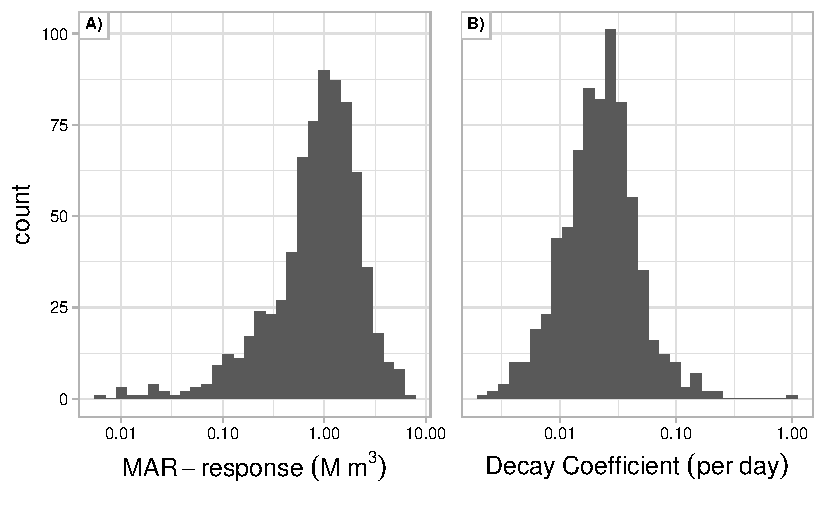
\includegraphics[keepaspectratio]{AqC6.3_paper2_V4_files/figure-pdf/fig-histogram-1.pdf}}

}

\caption{\label{fig-histogram}Distribution of the target variables, the
MAR-response, A, and the decay coefficient, B, based on 720 hypothetical
recharge sites.}

\end{figure}%

\subsubsection{Training process}\label{training-process}

U-Net is trained using the ADAM optimizer with a reducing learning rate
schedule with a relatively small batch size of 12. These settings have
been shown to effectively train the model (Fernandes et al., 2024). The
model was trained on the results from 500 recharge sites and its
performance was tracked during training using an unseen dataset,
validation set, of 100 recharge sites. The training was concluded if the
model performance didn't improve over ten epochs.

The training process for XGBoost follows a comprehensive approach aimed
at maximizing the performance and generalizability of the trained model.
The results of all the scenarios are divided into training (N = 500) and
testing sets (N = 220), which are used to train and assess the model's
generalization respectively. Employing repeated 10-fold cross-validation
with 5 repeats, the model hyperparameters are tuned systematically,
exploring a range of parameters such as tree depth, minimum node size,
and learning rate through a grid search methodology. Hyperparameters are
predefined settings in a machine learning model that control the
learning process, influencing how the model optimizes its predictions
and generalizes to new data. 500 values of each hyperparameter are
sampled with Latin Hypercube Sampling. This rigorous evaluation across
multiple folds mitigates overfitting and enhances reliability (Soper,
2021). The hyperparameters with the highest cross-validation
R\textsuperscript{2} were used to train the final model on the entire
training set resulting in a robust XGBoost regression model improving
the model's generalizability to out-of-sample scenarios.

\subsubsection{The effect of specific yield}\label{sec-methods-SY}

In addition to the listed inputs, the transient phreatic groundwater
heads are also dependent on the specific yield of the aquifer, unlike
for steady-state groundwater heads. The specific yield ranges between 0
and 1, which is a ratio between the flux into or out of the model cell
and the associated head change per unit area of the cell. It affects how
quickly the groundwater heads react to fluxes in the groundwater. While
the original inputs were selected based on Fernandes et al. (2024),
which focused on the steady-state groundwater response, this analysis
targets the transient response, where the specific yield plays a
critical role. For this study, the specific yield from the baseline
scenario with natural precipitation is used as an input, which was
calculated for each time step using the unsaturated zone model MetaSWAP
(part of the numerical model simulations). The time series of specific
yield was divided into two periods: summer and winter, just like the
groundwater depth data. The average winter specific yield is used to
predict the MAR-response while the summer specific yield is used for the
decay coefficient. The specific yield around the sites is represented
using a Gaussian filter, just like the other inputs.

\subsubsection{Interpreting the learnt
relations}\label{interpreting-the-learnt-relations}

SHAP (SHapley Additive exPlanations) values provide a comprehensive
method for interpreting machine learning models by attributing
importance values to each input feature (Lundberg \& Lee, 2017; Young,
1985). These values, derived from game theory principles, delineate the
impact of individual features on model predictions. Here we use Tree
SHAP (Lundberg et al., 2020), which is optimized for tree-based machine
learning models such as XGBoost. Positive SHAP values indicate that a
feature increases the predicted target, while negative values indicate a
decrease. Importantly, the sum of all SHAP values for each feature
equals the predicted target variable, as expressed in
Equation~\ref{eq-SHAP_add}:

\begin{equation}\phantomsection\label{eq-SHAP_add}{
\hat{y} = \hat{y_0} + S_{x_1} + S_{x_2} + \dots + S_{x_n}
}\end{equation}

where \(\hat{y}\) is the predicted target, \(\hat{y_0}\) is the average
target across the training dataset, and \(S_{x_1}\), \(S_{x_2}\),
\ldots{} \(S_{x_n}\) are the SHAP values of the input features.

In this study, the target variables (MAR-response and decay coefficient)
are log-transformed before training the model and the SHAP values
explain the predictions on the log-transformed scale. To interpret the
SHAP values in the original scale of the target variables, they are
inverse-transformed by exponentiation. As per the product rule of
exponents, this transformation converts the SHAP values from being
additive to multiplicative, as shown in Equation~\ref{eq-SHAP_prod}. In
this transformed context, \(10^{\hat{y_0}}\) approximates the average
target value in the original scale. Here, a SHAP value of 1.5 indicates
that the feature increases the prediction by 1.5 times, or 50\% higher
than the average target value \(10^{\hat{y_0}}\).

\begin{equation}\phantomsection\label{eq-SHAP_prod}{
10^\hat{y} = 10^\hat{y_0} \cdot 10^{S_{x_1}} \cdot 10^{S_{x_2}} \cdot \dots \cdot 10^{S_{x_n}}
}\end{equation}

\subsection{Efficient locations for
MAR}\label{efficient-locations-for-mar}

The trained ML models were used to calculate many recharge sites across
the entire model domain to identify efficient MAR-locations. To maintain
comparability, the size and the recharge rate at the sites are
maintained between them to be 10 ha and 15 mm/day respectively. In
total, 1.6 million recharge sites were simulated with a space of 25 m
between their centres, which corresponds to the resolution of the
geo-hydrological data. The locations are compared based on three
criteria, the steady-state MAR-response, the MAR-response after 5 months
of artificial recharge and the fraction of the MAR-response left in the
subsurface after 3 months of no recharge. The steady-state MAR-response
is estimated using the U-Net from Fernandes et al. (2024), while the
transient MAR-response, ie. after 5 months of recharge, is estimated
using XGBoost for its faster estimates than U-Net. Similarly the
fraction is calculated from the decay coefficient from XGBoost using
Equation~\ref{eq-linear-reservoir-dqS}. We calculate the fraction to
demonstrate the versatility of the decay coefficient. As it is
independent of the duration it allows the user to define the duration of
the dry period they are interested in.

\section{Results}\label{results}

\subsection{MAR-response estimates}\label{mar-response-estimates}

\subsubsection{Steady-state estimates}\label{steady-state-estimates}

When estimating the MAR-response, the groundwater response at the end of
the recharge period, the steady state response could be a rather quick
estimate that is simulated using the numerical groundwater model. It
represents the result of long-term artificial recharge. However,
seasonal variations and the short recharge period make this estimate
inaccurate. The steady-state response typically exceeds the transient
MAR-response for the majority of recharge sites, as illustrated in
Figure~\ref{fig-response_ts} A and Figure~\ref{fig-y_yhat_steady}. On
average, the transient MAR-response was 56\% of the steady-state
response, between 37\% and 79\% for 90\% of the sites. Additionally, 10
sites exhibited a higher MAR-response than the steady-state response,
one of which is depicted in Figure~\ref{fig-response_ts} A. This can be
attributed to lower groundwater heads in February, near these recharge
sites, compared to steady-state conditions due to the high
transmissivity and proximity to streams and rivers. However, the
transient MAR-response shows a strong correlation with the steady-state
response, with an R\textsuperscript{2} of 0.92. This suggests that the
steady-state response can serve as a good proxy to identify locations
where MAR is likely to result in a high MAR-response. However,
steady-state estimates do not provide precise quantification of the
response, nor do they offer insights into the duration for which the
stored water will remain in the subsurface. Addressing these questions
requires simulating transient scenarios.

\begin{figure}

\centering{

\pandocbounded{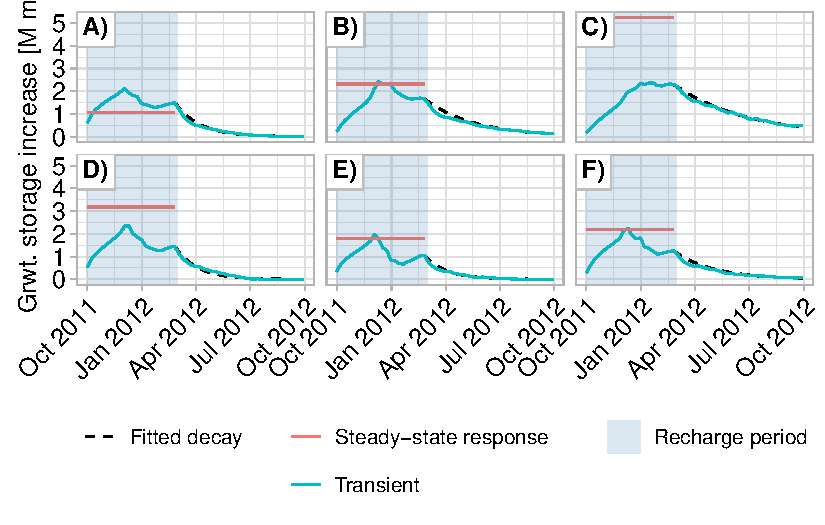
\includegraphics[keepaspectratio]{AqC6.3_paper2_V4_files/figure-pdf/fig-response_ts-1.pdf}}

}

\caption{\label{fig-response_ts}Groundwater response simulated at six
hypothetical recharge sites. The steady state and the transient response
are calculated from scenarios simulated with the numerical groundwater
model AMIGO while the fitted decay is fit using a robust linear
regression.}

\end{figure}%

\begin{figure}

\centering{

\pandocbounded{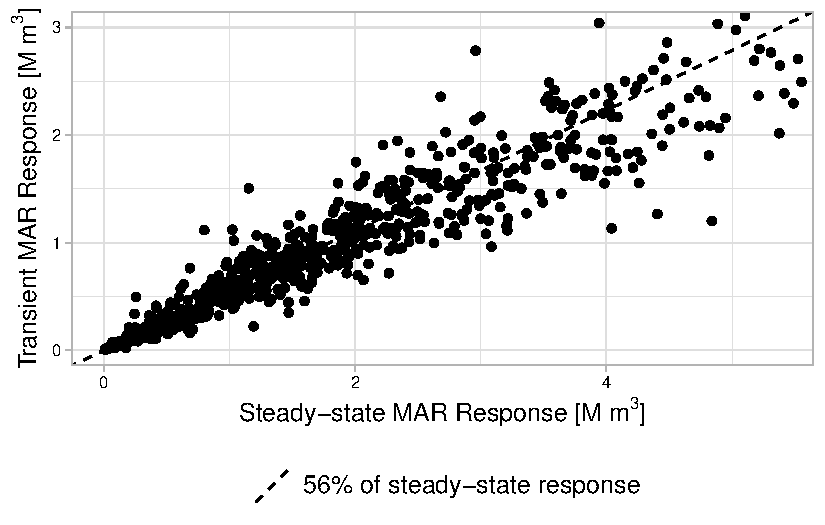
\includegraphics[keepaspectratio]{AqC6.3_paper2_V4_files/figure-pdf/fig-y_yhat_steady-1.pdf}}

}

\caption{\label{fig-y_yhat_steady}The volume of Steady-state response as
compared to the transient MAR-response on 25th February, after five
months of artificial recharge. Both responses are estimated using the
numerical groundwater model. The dotted line represents the average
ratio of the MAR-response to the steady-state response.}

\end{figure}%

\begin{figure}

\begin{minipage}{\linewidth}

\pandocbounded{\includegraphics[keepaspectratio]{Z:/stationary_res_AMIGO/png/rch_79_l1.png}}

\end{minipage}%

\caption{\label{fig-diff_steady}The response (change in groundwater
head) to 5 months of artificial recharge, transient MAR-response (A) and
the steady-state response (B) in cm based on the numerical model
simulation. C illustrates the increase in the steady-state response
relative to the transient MAR-response (B-A). The percent of the
steady-state response achieved after recharging for five months is
represented in D with the symmetric mean absolute error
(\(\frac{B-A}{(B+A)/2} \cdot 100\)).}

\end{figure}%

\subsubsection{Machine Learning
estimates}\label{machine-learning-estimates}

XGBoost predicts the volume of the transient MAR-response based on the
recharge rate applied at the site and averaged geo-hydrological
properties around the site, as described in
Section~\ref{sec-data-preparation}. The MAR-response typically falls
within 81\% to 144\% (10\textsuperscript{th} and 90\textsuperscript{th}
percentile) of the response simulated with the numerical model. XGBoost
is more accurate at predicting low MAR-response while underestimating
high response (Figure~\ref{fig-y-y_hat_all} B). This could be due to the
log transformation of the MAR-response before training the XGBoost
model. Transforming the response helps reduce the bias in the trained
model due to the right skew in the distribution of the MAR-response from
the simulated scenarios. Even though the predictions show bias, XGBoost
performs well overall, achieving a Mean Absolute Error (MAE) of 0.22 M
m\textsuperscript{3} (million m\textsuperscript{3}), a Mean Absolute
Percent Error (MAPE) of 18.68\% with a coefficient of determination
(R\textsuperscript{2}) of 0.84.

U-Net predicts the response in each cell in the catchment based on 2-D
inputs of geo-hydrological properties. Unlike the Gaussian kernel used
to represent the properties around the recharge sites for XGBoost, U-Net
learns to extract relevant features of the inputs during the model
training process. The MAR-response simulated by the numerical model
ranges between 82\% and 164\%of the predicted response by U-net.
However, U-Net tends to underestimate low responses, as observed in four
of the 120 sites tested. When focusing on sites with responses greater
than 0.25 M m3, the upper bound of the range decreases significantly
from 164\% to 135\%, indicating a better accuracy for large responses.
Despite these occasional inaccuracies, particularly for low responses,
U-Net achieves better overall performance than XGBoost, with a MAE of
0.16 M m\textsuperscript{3}, a MAPE of 18.84\%, and an
R\textsuperscript{2} of 0.93.

\begin{figure}

\centering{

\pandocbounded{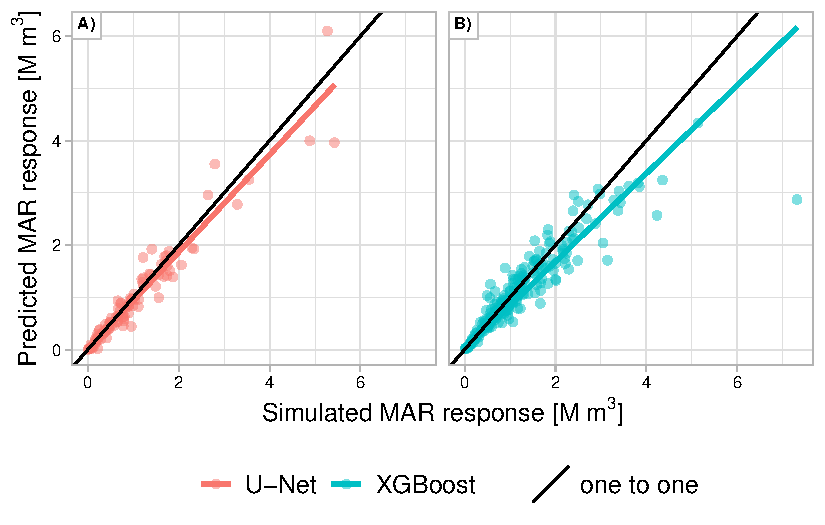
\includegraphics[keepaspectratio]{AqC6.3_paper2_V4_files/figure-pdf/fig-y-y_hat_all-1.pdf}}

}

\caption{\label{fig-y-y_hat_all}Modelled vs Predicted MAR-response for
recharge sites used to test the ML models. A linear fit through the
points, coloured dotted line, is added in the plot depicting the trend
of the points along with a black solid line showing one-one relation.}

\end{figure}%

\subsubsection{Informative features}\label{informative-features}

Obviously, among the inputs, the recharge site area and the recharge
rate have the most substantial impact on the MAR-response, as
illustrated in Figure~\ref{fig-SHAPintial_response2}. This is evident
from the wide range of SHAP values for these inputs to the XGBoost
model. A high recharge rate and large site area correspond with a
greater MAR-response, as expected, given the larger volume of water to
be recharged from these sites. Additionally, among the other properties,
the surface water network and the groundwater depth explain most of the
variation in the MAR-response. Transmissivity, vertical resistance and
drain conductance have the least impact on the MAR-response.
Furthermore, all inputs are positively correlated with the MAR-response
except for the properties of the surface water network - river density,
river conductance, and drain conductance, as seen in
Figure~\ref{fig-SHAPintial_response2}, which in general means that more
extensive drainage networks leads to lower MAR response.

The SHAP values of the MAR-response show a near-linear relation to the
site design parameters, area of the recharge site and recharge rate
applied at the site (Figure~\ref{fig-SHAPintial_response2} A and B).
These parameters affect the total recharge volume applied, which is a
product of the recharge rate and the area of the recharge site.
Logically, a higher total recharge would lead to a larger response as
reflected in the identified relation. However, the effect of increasing
the size of the recharge site is not perfectly linear but it shows a
decreasing benefit, especially for sites larger than 0.5
km\textsuperscript{2} (Figure~\ref{fig-Analyze_site_area} A). Similarly,
increasing the recharge rate beyond 15 mm/day shows a decreasing benefit
in the response (Figure~\ref{fig-Analyze_site_area} B). This suggests
that multiple small sites could be more beneficial to maximize the water
stored in the subsurface than a single large recharge site.

Following the site design parameters, the properties of the surface
water network have the biggest impact on the MAR-response
(Figure~\ref{fig-SHAPintial_response2} C, E and H). Low river density is
related to a high MAR-response, resulting in a maximum of 50\% higher
response than the average recharge site simulated. A higher river
density than 0.05 leads to a decreasing response, with a rapid initial
decrease which gradually reaches a minimum. Sites with a river density
of more than 0.2 have 10 to 20\% lower response than a site with a river
density of 0.1. Together this indicates that an extensive surface water
network more effectively drains the recharged water, diminishing the
MAR-response. River conductance also has a similar impact, with sites
near streams with a river bottom conductance of less than 2 m2/day
having a 20\% higher MAR-response. The MAR-response then decreases
exponentially with increasing river conductance, up to 15 m2/day. A high
river conductance leads to a similarly low response of 30\% lower
MAR-response than the average predicted MAR-response, \(10^{\hat{y}_0}\)
in equation Equation~\ref{eq-SHAP_prod}. These high river conductances
are primarily associated with large rivers due to their larger wetted
perimeter, resulting in a much larger draining capacity. Tile drainage
has a minor impact on the response, ranging from 5\% higher to 10\%
lower MAR-response. Recharge sites near fields with a low drain
conductance have a higher MAR-response than those with a higher drain
conductance. However, fields with tile drainage are not common in the
study area decreasing the reliability of the identified relation.

The groundwater depth is a unique input feature as it is the result of
groundwater flow that is determined by multiple system characteristics,
such as river density, river stage, and transmissivity. It also
determines the available storage space for the MAR-response, acting as a
limiting factor when groundwater levels are within 3 m
(Figure~\ref{fig-SHAPintial_response2} E). The MAR-response at these
sites varies between 20\% lower to 40\% higher than the average
predicted MAR-response. Interestingly, about 95\% of the recharge sites
have a maximum head increase of less than 3 m. It is worth noting that
this characteristic of the response was not known by the model apriori,
but was identified while being trained to predict a different target. In
areas with deeper groundwater levels, groundwater depth has minimal
impact on the MAR-response.

While it is possible that the groundwater heads do not increase beyond 3
m within five months of artificial recharge due to the recharge rates
considered and the transmissivity of the aquifer, it is most likely a
result of the characteristics of the groundwater depth within the study
area. The groundwater is within 3 m from the ground level in 98\% of the
study area. Applying a similar methodology at another study area with
deeper groundwater levels would likely show a continuation of the linear
trend identified. Based on this, we can extrapolate that sites with
deeper groundwater levels are always preferred when selecting artificial
recharge sites.

Among the inputs compared, the aquifer properties have the smallest
impact on the MAR-response (Figure~\ref{fig-SHAPintial_response2} F and
G). In general, MAR-response increases with transmissivity as it enables
the spread of the response away from the recharge site, saturating a
wider extent of the aquifer. Sites in poorly transmissive soil can have
up to 15\% lower MAR-response than the average predicted MAR-response,
while moderate transmissivity, 250 m2/day to 1000 m2/day has a 5 to 10\%
lower response. The MAR-response increases for more transmissive
aquifers, up to 1300 m2/day, resulting in up to 7.5\% higher response.
Further increases in transmissivity, up to 3000 m2/day, has a minor
impact on the response. Vertical resistance has a minor but highly
non-linear impact on the response, with low vertical resistance related
to a smaller MAR-response, up to 8\% lower response, and high resistance
resulting in a high MAR-response, up to 8\% higher.

\begin{figure}

\centering{

\pandocbounded{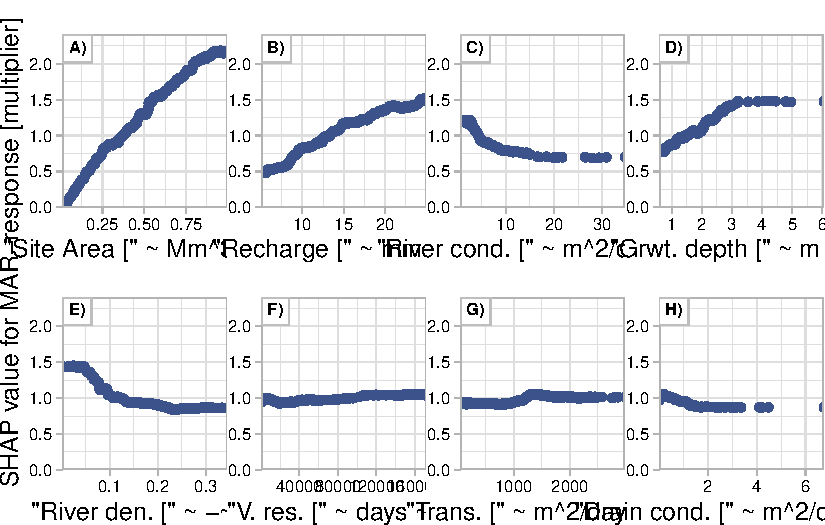
\includegraphics[keepaspectratio]{AqC6.3_paper2_V4_files/figure-pdf/fig-SHAPintial_response2-1.pdf}}

}

\caption{\label{fig-SHAPintial_response2}Variation in SHAP value across
each input to the XGBoost model. Each point represents a recharge site
in the training dataset.}

\end{figure}%

\subsubsection{Effect of Specific yield on the
MAR-response}\label{effect-of-specific-yield-on-the-mar-response}

Including specific yield as an input improved the predictability of the
MAR-response. This is a reflection of this input's importance in
transient scenarios. Interestingly, including specific yield improved
the Root Mean Squared Error, RMSE, more than the Mean Absolute Error,
MAE, and the Mean Absolute Percent Error, MAPE. As RMSE is more
sensitive to large errors, adding specific yield especially reduced
these errors suggesting that the model trained with specific yield makes
fewer or smaller large errors. Since achieving a high MAR-response is a
desirable outcome when optimizing MAR sites, these improvements are
particularly beneficial for improving the model's predictive power.

\global\setlength{\Oldarrayrulewidth}{\arrayrulewidth}

\global\setlength{\Oldtabcolsep}{\tabcolsep}

\setlength{\tabcolsep}{2pt}

\renewcommand*{\arraystretch}{1.5}



\providecommand{\ascline}[3]{\noalign{\global\arrayrulewidth #1}\arrayrulecolor[HTML]{#2}\cline{#3}}

\begin{longtable}[c]{ccccccccc}

\caption{\label{tbl-xgb_performance_sto}Model performance when including
Specific Yield (SY) as an input to the model.}

\tabularnewline

\ascline{1.5pt}{666666}{1-9}

\multicolumn{1}{!{\color[HTML]{666666}\vrule width 1pt}>{}c}{\textcolor[HTML]{000000}{\fontsize{11}{11}\selectfont{\global\setmainfont{Arial}{\textbf{Inputs}}}}} & \multicolumn{4}{!{\color[HTML]{666666}\vrule width 1pt}>{}c}{\textcolor[HTML]{000000}{\fontsize{11}{11}\selectfont{\global\setmainfont{Arial}{\textbf{MAR-response}}}}} & \multicolumn{4}{!{\color[HTML]{666666}\vrule width 1pt}>{}c!{\color[HTML]{666666}\vrule width 1pt}}{\textcolor[HTML]{000000}{\fontsize{11}{11}\selectfont{\global\setmainfont{Arial}{\textbf{Decay\ Coefficient}}}}} \\





\multicolumn{1}{!{\color[HTML]{666666}\vrule width 1pt}>{}l}{\textcolor[HTML]{000000}{\fontsize{11}{11}\selectfont{\global\setmainfont{Arial}{\textbf{}}}}} & \multicolumn{1}{!{\color[HTML]{666666}\vrule width 1pt}>{}r}{\textcolor[HTML]{000000}{\fontsize{11}{11}\selectfont{\global\setmainfont{Arial}{\textbf{RMSE}}}}} & \multicolumn{1}{>{}r}{\textcolor[HTML]{000000}{\fontsize{11}{11}\selectfont{\global\setmainfont{Arial}{\textbf{R}}}}\textcolor[HTML]{000000}{\fontsize{11}{11}\selectfont{\global\setmainfont{Arial}{\textbf{\textsuperscript{2}}}}}} & \multicolumn{1}{>{}r}{\textcolor[HTML]{000000}{\fontsize{11}{11}\selectfont{\global\setmainfont{Arial}{\textbf{MAPE}}}}} & \multicolumn{1}{>{}r}{\textcolor[HTML]{000000}{\fontsize{11}{11}\selectfont{\global\setmainfont{Arial}{\textbf{MAE}}}}} & \multicolumn{1}{!{\color[HTML]{666666}\vrule width 1pt}>{}r}{\textcolor[HTML]{000000}{\fontsize{11}{11}\selectfont{\global\setmainfont{Arial}{\textbf{RMSE}}}}} & \multicolumn{1}{>{}r}{\textcolor[HTML]{000000}{\fontsize{11}{11}\selectfont{\global\setmainfont{Arial}{\textbf{R}}}}\textcolor[HTML]{000000}{\fontsize{11}{11}\selectfont{\global\setmainfont{Arial}{\textbf{\textsuperscript{2}}}}}} & \multicolumn{1}{>{}r}{\textcolor[HTML]{000000}{\fontsize{11}{11}\selectfont{\global\setmainfont{Arial}{\textbf{MAPE}}}}} & \multicolumn{1}{>{}r!{\color[HTML]{666666}\vrule width 1pt}}{\textcolor[HTML]{000000}{\fontsize{11}{11}\selectfont{\global\setmainfont{Arial}{\textbf{MAE}}}}} \\

\ascline{1.5pt}{666666}{1-9}\endfirsthead 

\ascline{1.5pt}{666666}{1-9}

\multicolumn{1}{!{\color[HTML]{666666}\vrule width 1pt}>{}c}{\textcolor[HTML]{000000}{\fontsize{11}{11}\selectfont{\global\setmainfont{Arial}{\textbf{Inputs}}}}} & \multicolumn{4}{!{\color[HTML]{666666}\vrule width 1pt}>{}c}{\textcolor[HTML]{000000}{\fontsize{11}{11}\selectfont{\global\setmainfont{Arial}{\textbf{MAR-response}}}}} & \multicolumn{4}{!{\color[HTML]{666666}\vrule width 1pt}>{}c!{\color[HTML]{666666}\vrule width 1pt}}{\textcolor[HTML]{000000}{\fontsize{11}{11}\selectfont{\global\setmainfont{Arial}{\textbf{Decay\ Coefficient}}}}} \\





\multicolumn{1}{!{\color[HTML]{666666}\vrule width 1pt}>{}l}{\textcolor[HTML]{000000}{\fontsize{11}{11}\selectfont{\global\setmainfont{Arial}{\textbf{}}}}} & \multicolumn{1}{!{\color[HTML]{666666}\vrule width 1pt}>{}r}{\textcolor[HTML]{000000}{\fontsize{11}{11}\selectfont{\global\setmainfont{Arial}{\textbf{RMSE}}}}} & \multicolumn{1}{>{}r}{\textcolor[HTML]{000000}{\fontsize{11}{11}\selectfont{\global\setmainfont{Arial}{\textbf{R}}}}\textcolor[HTML]{000000}{\fontsize{11}{11}\selectfont{\global\setmainfont{Arial}{\textbf{\textsuperscript{2}}}}}} & \multicolumn{1}{>{}r}{\textcolor[HTML]{000000}{\fontsize{11}{11}\selectfont{\global\setmainfont{Arial}{\textbf{MAPE}}}}} & \multicolumn{1}{>{}r}{\textcolor[HTML]{000000}{\fontsize{11}{11}\selectfont{\global\setmainfont{Arial}{\textbf{MAE}}}}} & \multicolumn{1}{!{\color[HTML]{666666}\vrule width 1pt}>{}r}{\textcolor[HTML]{000000}{\fontsize{11}{11}\selectfont{\global\setmainfont{Arial}{\textbf{RMSE}}}}} & \multicolumn{1}{>{}r}{\textcolor[HTML]{000000}{\fontsize{11}{11}\selectfont{\global\setmainfont{Arial}{\textbf{R}}}}\textcolor[HTML]{000000}{\fontsize{11}{11}\selectfont{\global\setmainfont{Arial}{\textbf{\textsuperscript{2}}}}}} & \multicolumn{1}{>{}r}{\textcolor[HTML]{000000}{\fontsize{11}{11}\selectfont{\global\setmainfont{Arial}{\textbf{MAPE}}}}} & \multicolumn{1}{>{}r!{\color[HTML]{666666}\vrule width 1pt}}{\textcolor[HTML]{000000}{\fontsize{11}{11}\selectfont{\global\setmainfont{Arial}{\textbf{MAE}}}}} \\

\ascline{1.5pt}{666666}{1-9}\endhead



\multicolumn{9}{!{\color[HTML]{666666}\vrule width 1pt}>{}c!{\color[HTML]{666666}\vrule width 1pt}}{\textcolor[HTML]{000000}{\fontsize{11}{11}\selectfont{\global\setmainfont{Arial}{Head\ Response}}}} \\

\ascline{0.75pt}{666666}{1-9}



\multicolumn{1}{!{\color[HTML]{666666}\vrule width 1pt}>{}l}{\textcolor[HTML]{000000}{\fontsize{11}{11}\selectfont{\global\setmainfont{Arial}{Without\ SY}}}} & \multicolumn{1}{!{\color[HTML]{666666}\vrule width 1pt}>{}r}{\textcolor[HTML]{000000}{\fontsize{11}{11}\selectfont{\global\setmainfont{Arial}{0.4360}}}} & \multicolumn{1}{>{}r}{\textcolor[HTML]{000000}{\fontsize{11}{11}\selectfont{\global\setmainfont{Arial}{0.84}}}} & \multicolumn{1}{>{}r}{\textcolor[HTML]{000000}{\fontsize{11}{11}\selectfont{\global\setmainfont{Arial}{19}}}} & \multicolumn{1}{>{}r}{\textcolor[HTML]{000000}{\fontsize{11}{11}\selectfont{\global\setmainfont{Arial}{0.2240}}}} & \multicolumn{1}{!{\color[HTML]{666666}\vrule width 1pt}>{}r}{\textcolor[HTML]{000000}{\fontsize{11}{11}\selectfont{\global\setmainfont{Arial}{0.00427}}}} & \multicolumn{1}{>{}r}{\textcolor[HTML]{000000}{\fontsize{11}{11}\selectfont{\global\setmainfont{Arial}{0.80}}}} & \multicolumn{1}{>{}r}{\textcolor[HTML]{000000}{\fontsize{11}{11}\selectfont{\global\setmainfont{Arial}{16}}}} & \multicolumn{1}{>{}r!{\color[HTML]{666666}\vrule width 1pt}}{\textcolor[HTML]{000000}{\fontsize{11}{11}\selectfont{\global\setmainfont{Arial}{0.00251}}}} \\

\ascline{0.75pt}{666666}{1-9}



\multicolumn{1}{!{\color[HTML]{666666}\vrule width 1pt}>{}l}{\textcolor[HTML]{000000}{\fontsize{11}{11}\selectfont{\global\setmainfont{Arial}{With\ SY}}}} & \multicolumn{1}{!{\color[HTML]{666666}\vrule width 1pt}>{}r}{\textcolor[HTML]{000000}{\fontsize{11}{11}\selectfont{\global\setmainfont{Arial}{0.3700}}}} & \multicolumn{1}{>{}r}{\textcolor[HTML]{000000}{\fontsize{11}{11}\selectfont{\global\setmainfont{Arial}{0.88}}}} & \multicolumn{1}{>{}r}{\textcolor[HTML]{000000}{\fontsize{11}{11}\selectfont{\global\setmainfont{Arial}{18}}}} & \multicolumn{1}{>{}r}{\textcolor[HTML]{000000}{\fontsize{11}{11}\selectfont{\global\setmainfont{Arial}{0.2020}}}} & \multicolumn{1}{!{\color[HTML]{666666}\vrule width 1pt}>{}r}{\textcolor[HTML]{000000}{\fontsize{11}{11}\selectfont{\global\setmainfont{Arial}{0.00395}}}} & \multicolumn{1}{>{}r}{\textcolor[HTML]{000000}{\fontsize{11}{11}\selectfont{\global\setmainfont{Arial}{0.82}}}} & \multicolumn{1}{>{}r}{\textcolor[HTML]{000000}{\fontsize{11}{11}\selectfont{\global\setmainfont{Arial}{13}}}} & \multicolumn{1}{>{}r!{\color[HTML]{666666}\vrule width 1pt}}{\textcolor[HTML]{000000}{\fontsize{11}{11}\selectfont{\global\setmainfont{Arial}{0.00220}}}} \\

\ascline{0.75pt}{666666}{1-9}



\multicolumn{9}{!{\color[HTML]{666666}\vrule width 1pt}>{}c!{\color[HTML]{666666}\vrule width 1pt}}{\textcolor[HTML]{000000}{\fontsize{11}{11}\selectfont{\global\setmainfont{Arial}{Water\ Stored\ in\ Response}}}} \\

\ascline{0.75pt}{666666}{1-9}



\multicolumn{1}{!{\color[HTML]{666666}\vrule width 1pt}>{}l}{\textcolor[HTML]{000000}{\fontsize{11}{11}\selectfont{\global\setmainfont{Arial}{Without\ SY}}}} & \multicolumn{1}{!{\color[HTML]{666666}\vrule width 1pt}>{}r}{\textcolor[HTML]{000000}{\fontsize{11}{11}\selectfont{\global\setmainfont{Arial}{0.0745}}}} & \multicolumn{1}{>{}r}{\textcolor[HTML]{000000}{\fontsize{11}{11}\selectfont{\global\setmainfont{Arial}{0.80}}}} & \multicolumn{1}{>{}r}{\textcolor[HTML]{000000}{\fontsize{11}{11}\selectfont{\global\setmainfont{Arial}{23}}}} & \multicolumn{1}{>{}r}{\textcolor[HTML]{000000}{\fontsize{11}{11}\selectfont{\global\setmainfont{Arial}{0.0350}}}} & \multicolumn{1}{!{\color[HTML]{666666}\vrule width 1pt}>{}r}{\textcolor[HTML]{000000}{\fontsize{11}{11}\selectfont{\global\setmainfont{Arial}{0.01310}}}} & \multicolumn{1}{>{}r}{\textcolor[HTML]{000000}{\fontsize{11}{11}\selectfont{\global\setmainfont{Arial}{0.78}}}} & \multicolumn{1}{>{}r}{\textcolor[HTML]{000000}{\fontsize{11}{11}\selectfont{\global\setmainfont{Arial}{26}}}} & \multicolumn{1}{>{}r!{\color[HTML]{666666}\vrule width 1pt}}{\textcolor[HTML]{000000}{\fontsize{11}{11}\selectfont{\global\setmainfont{Arial}{0.00617}}}} \\

\ascline{0.75pt}{666666}{1-9}



\multicolumn{1}{!{\color[HTML]{666666}\vrule width 1pt}>{}l}{\textcolor[HTML]{000000}{\fontsize{11}{11}\selectfont{\global\setmainfont{Arial}{With\ SY}}}} & \multicolumn{1}{!{\color[HTML]{666666}\vrule width 1pt}>{}r}{\textcolor[HTML]{000000}{\fontsize{11}{11}\selectfont{\global\setmainfont{Arial}{0.0627}}}} & \multicolumn{1}{>{}r}{\textcolor[HTML]{000000}{\fontsize{11}{11}\selectfont{\global\setmainfont{Arial}{0.85}}}} & \multicolumn{1}{>{}r}{\textcolor[HTML]{000000}{\fontsize{11}{11}\selectfont{\global\setmainfont{Arial}{21}}}} & \multicolumn{1}{>{}r}{\textcolor[HTML]{000000}{\fontsize{11}{11}\selectfont{\global\setmainfont{Arial}{0.0305}}}} & \multicolumn{1}{!{\color[HTML]{666666}\vrule width 1pt}>{}r}{\textcolor[HTML]{000000}{\fontsize{11}{11}\selectfont{\global\setmainfont{Arial}{0.01300}}}} & \multicolumn{1}{>{}r}{\textcolor[HTML]{000000}{\fontsize{11}{11}\selectfont{\global\setmainfont{Arial}{0.77}}}} & \multicolumn{1}{>{}r}{\textcolor[HTML]{000000}{\fontsize{11}{11}\selectfont{\global\setmainfont{Arial}{22}}}} & \multicolumn{1}{>{}r!{\color[HTML]{666666}\vrule width 1pt}}{\textcolor[HTML]{000000}{\fontsize{11}{11}\selectfont{\global\setmainfont{Arial}{0.00572}}}} \\

\ascline{1.5pt}{666666}{1-9}


\end{longtable}

\arrayrulecolor[HTML]{000000}

\global\setlength{\arrayrulewidth}{\Oldarrayrulewidth}

\global\setlength{\tabcolsep}{\Oldtabcolsep}

\renewcommand*{\arraystretch}{1}

Based on the SHAP values, we can explain the effects of specific yield
on the relations identified by XGBoost. A high specific yield, more than
0.17, leads to a higher MAR-response, leading to an increase of up to
75\% of the average prediction. Sites where the specific yield exceeds
0.1 demonstrate a markedly higher MAR-response, changing from a 12\%
decrease to a 50\% increase for specific yields between 0.1 and 0.17.
However, this relation does not backed by theory, as a high specific
yield should lead to a smaller increase in the heads to the same
recharge. For a better explanation, a ML perspective could be
insightful. Specifically, the effect of multicollinearity becomes
apparent: the inclusion of specific yield reduced the importance of
groundwater depth and river density. These variables are correlated with
specific yield complicating the interpretation of the relations.
Locations with a shallow groundwater level are generally wetter due to
processes such as capillary rise (see Appendix 2) resulting in a lower
specific yield. The effect of these variables, groundwater depth and
river density, on the MAR-response can be explained in theory suggesting
that the large impact of specific yield is likely a result of the
specific yield being correlated with the other two features while also
being more closely correlated to the MAR-response. This would cause
XGBoost to over-emphasize the influence of the specific yield over the
two inputs with a direct relation.

Including specific yield as an input to the model thus reduced the
effect of river density on the MAR-response. Sites with a river density
of less than 0.05 have an up to 20\% higher MAR-response, which is a
reduction from a 40\% higher response based on the SHAP values from the
model that excludes specific yield from the inputs. As shown in Figures
16, and 17 in the Appendix, regions with a higher river density also
have the generally wetter condition in their root zone, reducing the
specific yield. On the contrary, deeper groundwater indicates dryer
conditions resulting in a higher specific yield. Areas with groundwater
levels deeper than 2.5 m have a 20\% higher MAR-response, which is a
reduction from a 50\% higher response based on the SHAP values from the
model that excludes specific yield. Interestingly, the limit identified
by XGBoost has also reduced from 3 m to 2.5 m depth with the inclusion
of specific yield.

Overall, including specific yield improves the accuracy of the model
even though the input is correlated with multiple other system
properties. This would likely have minimal influence on the
generalizability of the predictions from XGBoost as it is a decision
tree based model which is not affected by multicollinearity (Chen \&
Guestrin, 2016; Kotsiantis, 2013; Piramuthu, 2008). However, the learnt
relations are affected by multicollinearity, where the most informative
input is attributed with the highest importance. Based on the SHAP
values, river density and groundwater depth have a similar importance
while the specific yield has a higher importance than the two. This
suggests that while specific yield is the most informative input,
groundwater depth and river density have their independent influence on
the MAR-response.

\begin{figure}

\centering{

\pandocbounded{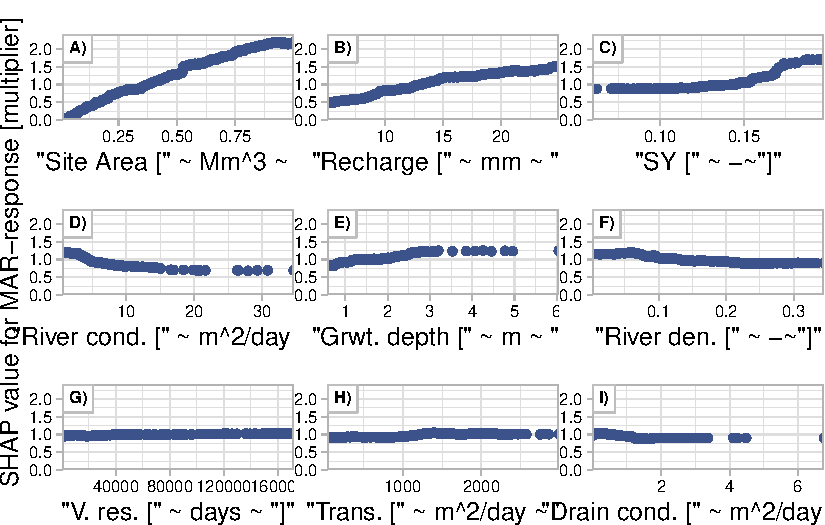
\includegraphics[keepaspectratio]{AqC6.3_paper2_V4_files/figure-pdf/fig-SHAPintial_response_po-1.pdf}}

}

\caption{\label{fig-SHAPintial_response_po}Variation in SHAP value
across each input to the XGBoost model trained with Specific Yield along
with other inputs. Each point represents a recharge site in the training
dataset.}

\end{figure}%

\subsection{Decay coefficient}\label{decay-coefficient}

The decay coefficient describes the rate at which the volume of extra
storage decreases over time per volume of extra storage, due to return
flow to the surface water network. As groundwater levels approach those
in the natural, baseline scenario, the drainage of groundwater gradually
decreases. In this study, artificial recharge is stopped on
1\textsuperscript{st} March 2012 and will resume from
1\textsuperscript{st} October 2012, representing 219 days without
artificial recharge. For example, if the decay coefficient is greater
than \(k = - \frac{\log 0.2} {219} \approx 0.0073\) per day, the stored
volume of water will decay to less than 20\% of the initial volume of
stored water at the end of the 219 days (see
Equation~\ref{eq-linear-reservoir-dqS}). It is important to note the
inverse relation between the decay coefficient and the water remaining
in the subsurface on 1st October 2012. Of the 720 randomly selected
hypothetical recharge sites used for training the model, only 52 have a
lower decay rate than 0.0073 per day. This emphasizes the importance of
optimization to identify site locations better suited for artificial
recharge.

\subsubsection{Machine Learning
estimates}\label{machine-learning-estimates-1}

XGBoost can accurately predict the decay rate of the modelled response.
The decay rate is within 79\% to 124\% of the predicted decay rate,
while not showing a systematic bias, as evidenced in
Figure~\ref{fig-y-y_hat_decay}. The MAE of the trained model is 0.0025
m, MAPE is 16\% and an R\textsuperscript{2} of 0.8. Relative to the
MAR-response, the decay coefficient proved to be more difficult to
predict. The model has a lower R\textsuperscript{2}, but also a lower
MAPE suggesting that while the model does not explain all the variance
in the data, it is more accurate at predicting low decay coefficient
resulting in a lower MAPE. This combination suggests that the trained
XGBoost models are especially accurate at identifying efficient recharge
sites, with high MAR-response and low decay coefficient.

\begin{figure}

\centering{

\pandocbounded{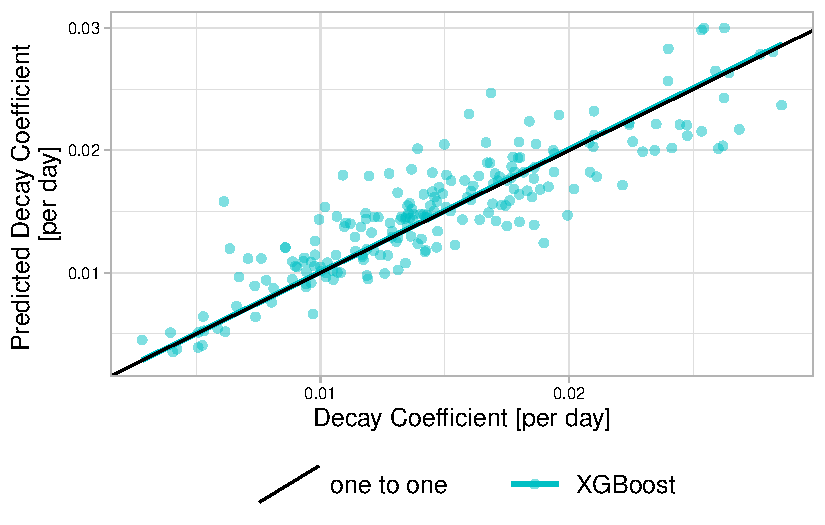
\includegraphics[keepaspectratio]{AqC6.3_paper2_V4_files/figure-pdf/fig-y-y_hat_decay-1.pdf}}

}

\caption{\label{fig-y-y_hat_decay}Modelled vs Predicted decay rate for
recharge sites used to test the models. A linear fit through the points,
coloured line, along with a black solid line showing one-one relation is
added in the plot depicting the trend of the points.}

\end{figure}%

\subsubsection{Informative features}\label{informative-features-1}

Different inputs are the most informative for the decay coefficient
relative to the MAR-response. The design parameters, which are the site
area and recharge rate, mostly have a minor effect on the decay
coefficient while they strongly affect the MAR-response. However, small
sites of less than 0.1 km2 have a drastically higher decay rate, as seen
in Figure~\ref{fig-SHAP-decay} A. To conceptualize this phenomenon that
affects the response in three dimensions in a two-dimensional framework,
the MAR-response can be likened to the area of a circle where the
surface water network acts on the perimeter of this circle. Larger
MAR-responses correspond to circles with greater areas. As the area
increases, the perimeter also expands, but at a slower rate relative to
the area. Consequently, larger MAR-responses are less influenced by
external factors, such as rivers and drains, much like how a larger
circle has a relatively smaller perimeter compared to its area. This
effect of small sites makes site area the third most important input
after groundwater depth and river conductance.

The average summer groundwater depth has the biggest impact on the decay
coefficient. Sites with a shallow groundwater level, of less than 1.5 m,
have a higher decay rate than the sites with deeper groundwater. After
groundwater depth, river conductance is the next most influential
variable. A low river conductance around the site is related to a lower
decay coefficient. Regions with an average river conductance of more
than 5 m\textsuperscript{2}/day have 25\% higher decay rate than the
average predicted decay coefficient. River density has a similar
relation, which is the fifth most influential variable.Regions with a
river density of more than 0.15 have a 5\% to 10\% higher decay
coefficient. Together these inputs capture a similar relation where
shallow groundwater level could cause the surface water network to be
more influential even for small increases in the groundwater level. The
groundwater stored at these locations is drained to the surface water as
a return flow, increasing the decay coefficient.

Aquifer properties have a bigger impact on the decay coefficient than on
the MAR-response. The vertical resistance below the top-most aquifer is
the fourth most impactful input. Regions with only one aquifer tend to
have a 5\% to 10\% lower decay coefficient, as in
Figure~\ref{fig-SHAP-decay} F. These locations are represented by a very
high vertical resistance of 171,000 days representing the basement
composed of the clayey Breda formation. Interestingly, the regions with
multiple aquifers have a 10\% higher decay coefficient. A low
transmissivity is associated with a lower decay coefficient,
Figure~\ref{fig-SHAP-decay} F. It decreases the spread of groundwater
resulting in lower drainage flux to the surrounding surface water
network. A transmissivity of more than 700 m2/day leads to a 5\% to 12\%
higher decay coefficient compared to the average predicted decay
coefficient (i.e.~SHAP = 1).

\begin{figure}

\centering{

\pandocbounded{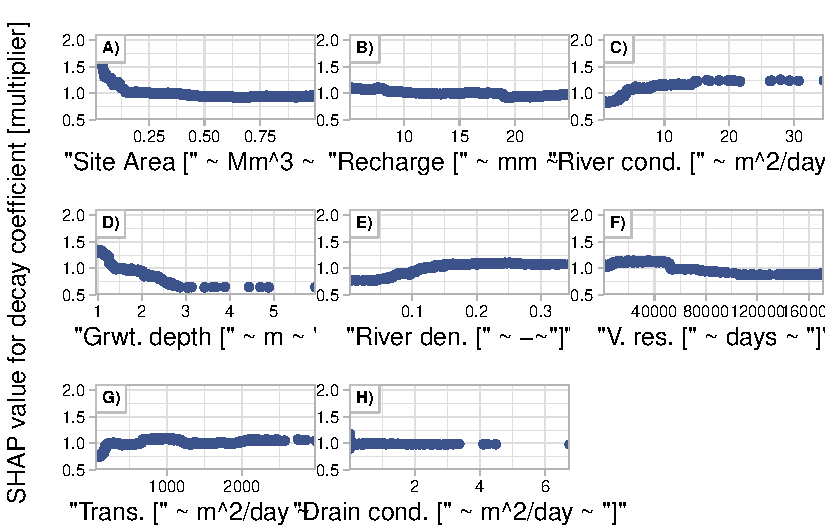
\includegraphics[keepaspectratio]{AqC6.3_paper2_V4_files/figure-pdf/fig-SHAP-decay-1.pdf}}

}

\caption{\label{fig-SHAP-decay}SHAP values of the inputs to the XGBoost
model for each recharge site used to test the model. SHAP values
\textgreater1 indicate that the feature at the recharge site contributed
to a higher decay coefficient. Conversely, negative SHAP values indicate
that the feature slowed the decay of the response.}

\end{figure}%

\subsubsection{Effect of Specific yield on the decay
coefficient}\label{effect-of-specific-yield-on-the-decay-coefficient}

Including the specific yield among the inputs improved the performance
of the model, see Table~\ref{tbl-xgb_performance_sto}. The model
improved on all metrics: RMSE, R\textsuperscript{2}, MAPE, and MAE by
between 8\% and 19\%. Interestingly, the MAE improved more than the RMSE
suggesting that the improvements are mostly at sites with a low decay
coefficient.

Sites with a high specific yield have a low decay coefficient. A high
specific yield decreases the reaction of groundwater heads to fluxes in
the groundwater. The same effect of specific yield also reduces the
decay of the response in the period without artificial recharge. XGBoost
identified this relation, predicting sites with a specific yield of less
than 0.1 have a 40\% higher decay coefficient. At the other extreme,
sites with a high specific yield of more than 0.19 have a 25\% lower
decay coefficient. The decay coefficient decreases linearly between
these two extremes. However, the constant effect at the extremes could
be due to the tree based architecture of XGBoost which results in lower
sensitivity at the extremes of the input features. A continuous linear
effect of specific yield could be expected if the model was trained with
more sites at these extremes.

As the specific yield is correlated to the groundwater depth and the
river density, the SHAP values for these two inputs are also affected.
The range of SHAP values related to these two inputs decreased compared
to the values for the model without specific yield, indicating a smaller
influence of these inputs. The effect of shallow groundwater decreased
dramatically due to the inclusion of specific yield among the inputs.
The low specific yield at locations with shallow groundwater explains
the suddenly higher decay coefficient at these sites. All sites with a
groundwater level within 2 m of the soil surface have a similar 10\%
higher decay coefficient . Based on the SHAP values, the river density
has almost no influence on the decay coefficient, suggesting that the
lower specific yield near the rivers explains most of the influence of
the river density.

\begin{figure}

\centering{

\pandocbounded{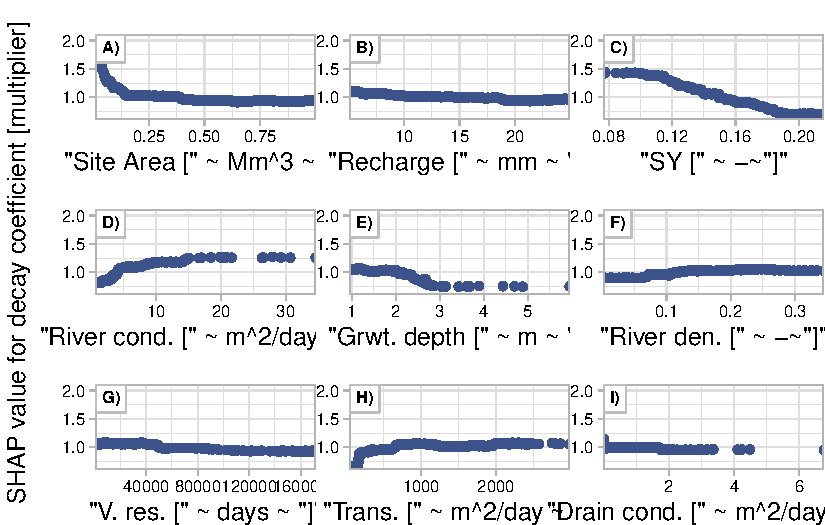
\includegraphics[keepaspectratio]{AqC6.3_paper2_V4_files/figure-pdf/fig-xgb_shap_por-1.pdf}}

}

\caption{\label{fig-xgb_shap_por}SHAP values of the inputs to the
XGBoost model trained with specific yield along with other inputs to the
model. Positive SHAP values indicate that the feature at the recharge
site contributed to a higher decay coefficient. Conversely, negative
SHAP values indicate that the feature reduced the decay rate.}

\end{figure}%

\subsection{Efficient locations for
MAR}\label{efficient-locations-for-mar-1}

The trained ML models, being computationally efficient, can be used to
estimate the groundwater response to MAR sites across the entire study
area, creating a regional scan of potential MAR sites,
Figure~\ref{fig-efficient_locations}. The two characteristics of the
groundwater storage were estimated at 1.6 million recharge sites that
were spaced at 25 m between their centers. These estimates were
completed within 20 seconds, demonstrating the efficiency of the ML
models. The surface network has a strong influence on the MAR-response
and the fraction of the response left over after 3 months. Both the
targets are reduced around the rivers to the west and the south-west,
except at the higher regions just north of the south-western river due
to the relatively deeper groundwater.

The area to the east especially shows a high potential for MAR, as
recharged water stays within the groundwater system for longer due to
the low transmissivity of the aquifer in this region. The area in the
centre shows a comparable initial MAR-response, but retains a smaller
fraction of water after three months, making the area less suitable for
MAR. While the steady-state response correlates well with both the
MAR-response and the fraction of water leftover, these results also show
that a transient approach is needed, as areas that might look promising
from a steady-state approach, appear to be less suitable in the more
realistic transient case.

\begin{figure}

\centering{

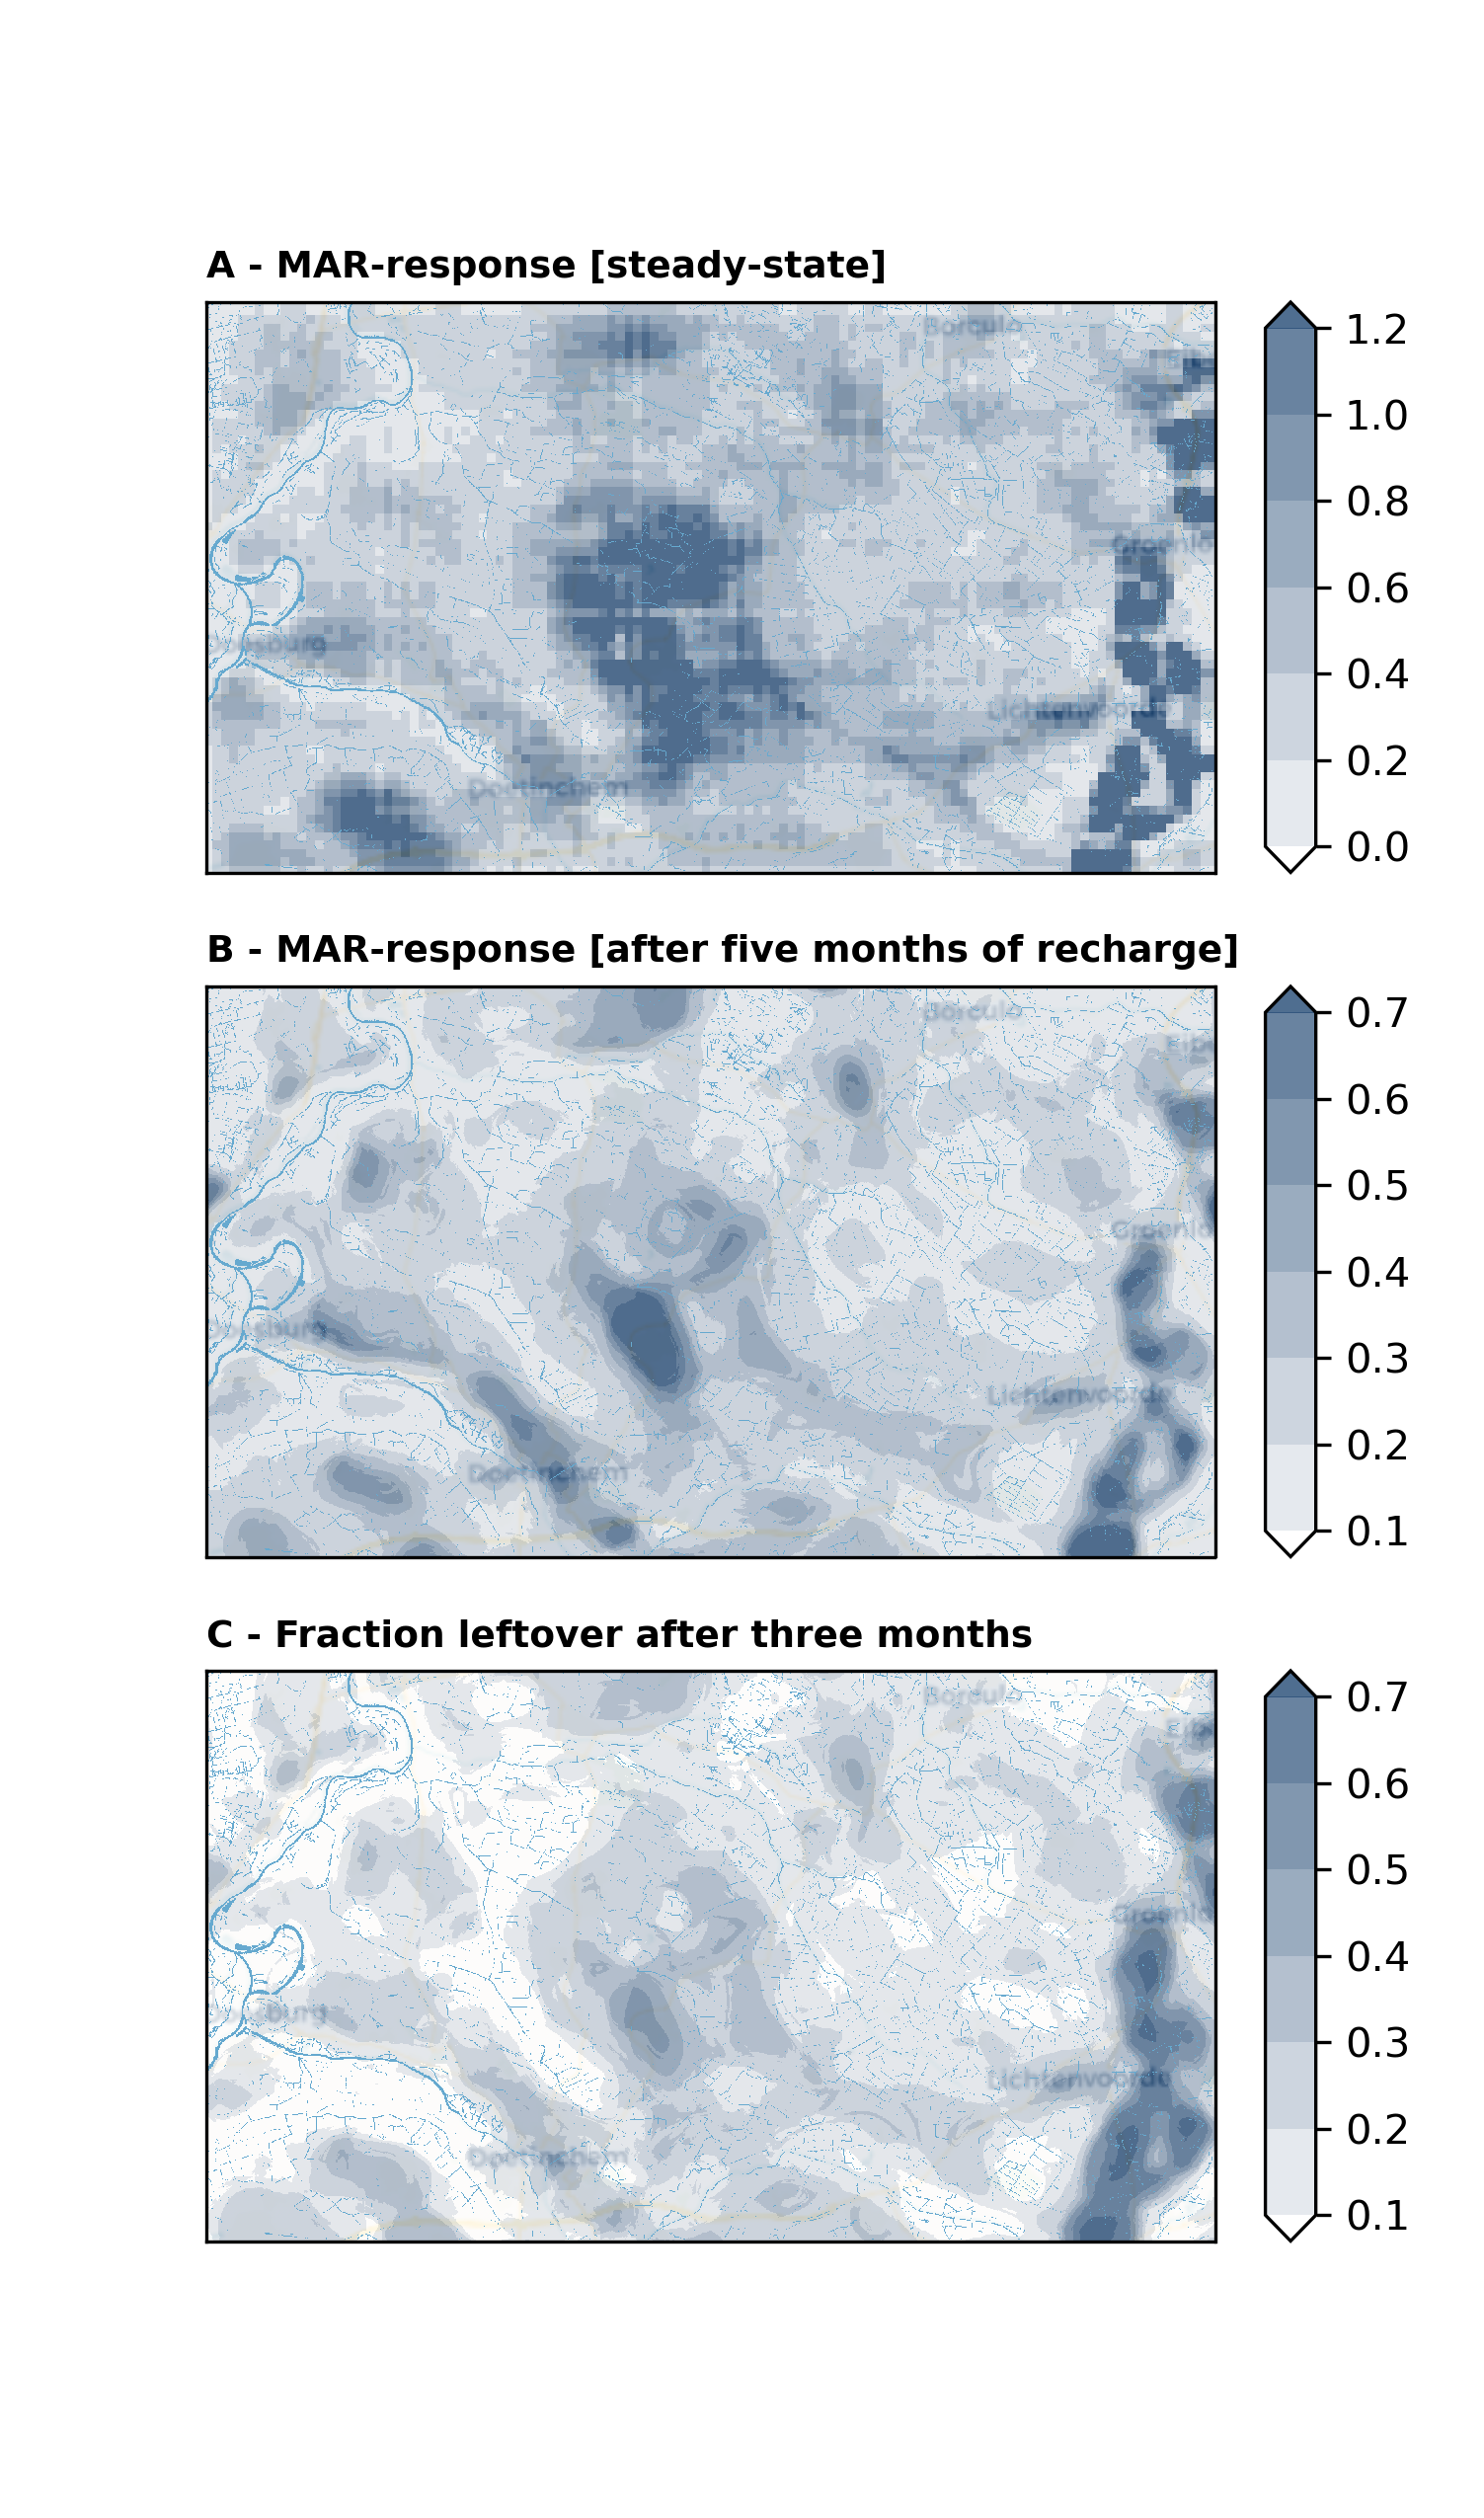
\includegraphics[width=10cm,height=\textheight,keepaspectratio]{C:/Users/valdf/MODFLOW_transient_res/predictions_with_steady_vertical.png}

}

\caption{\label{fig-efficient_locations}The groundwater response to 15
mm/day of artificial recharge applied over 10 ha recharge sites. The
steady-state MAR-response in million m3, A, is estimated using U-Net
(Fernandes et al., 2024) while the MAR-response after five months of
recharge in million m3, B, is estimated by XGBoost. The fraction of
water leftover {[}unit less{]}, C, is calculated from the decay
coefficient from XGBoost.}

\end{figure}%

\section{Discussion}\label{discussion}

Among the two ML techniques for estimating the MAR-response, U-Net
provides the most accurate estimate. It boasts a higher R2 value and a
lower MAPE. This better performance could be explained by U-Net's
ability to extract high-level features from the inputs in the encoder.
These features are not as physically interpretable as the Gaussian
kernel used to represent the features around the recharge site as used
in XGBoost. Furthermore, the Gaussian kernel is agnostic to the
orientation of features such as those of the surface water network. The
MAR-response would be higher if all streams were on the same side of the
recharge site than if the streams surrounded the site. A feature
extraction that can capture this relation could help improve XGBoost.
Techniques such as Gabbor filter, Fourier transform, and wavelet
transform could help better describe the density and orientation of the
surface water network. However, these filters extract multiple
representations, such as multiple frequencies in the case of Fourier
transformation, which would complicate model interpretability. So, there
is a trade-off to be made between the model complexity and the
interpretability of the ML model. Despite this disadvantage, the
Gaussian kernel has proved to adequately represent the properties around
the site while also maintaining a physical interpretation of being the
distance-weighted average which can be used to define a range of
influence of the feature on nearby recharge sites. Furthermore, as a
tree-based model, XGBoost is also more interpretable than U-Net, which
facilitates identifying and quantifying the effect of each of the inputs
on the MAR-response based on the SHAP values of the model. All
identified relations can be explained based on known theoretical
relations and the identified collinearity between the input features.

Site design decisions have the strongest influence on the expected
response of a system based on the SHAP values from XGBoost. A high
recharge rate applied over a large recharge site can effectively cause a
high MAR-response. While this is consistent with expectations, the
efficiency of the design decision cannot be commented on without
simulations. XGBoost identified that the efficiency of the recharge site
reduces for very high recharge rates suggesting multiple small sites
would be more efficient than a single large recharge site. Conversely,
the groundwater storage due to very small recharge sites decays faster
than larger sites. Overall, multiple recharge sites larger than 0.1 km2
each recharging up to 20 mm/day would offer the largest volume of
increased storage in the groundwater.

Favourable site properties can significantly enhance the expected
response. Of these properties, the surface network plays a pivotal role.
A low river density and river conductance greatly improve the long-term
groundwater storage associated with the recharge site. By strategically
reducing the number of small streams and their depths, water authorities
can reduce the river density and the river conductance and improve the
suitability of a site for desired outcomes. Thus, the interplay between
site design and surface network properties offers avenues for
manipulating locations to increase the effect of MAR and maximize the
stored water.

Among the aquifer properties, locations in a more transmissive aquifer
with deep groundwater are commonly identified as potential recharge
sites (Gibson \& Campana, 2014; LaHaye et al., 2021). These relations
are based on Brown et al. (2005) who determined 450 m2/day to 2300
m2/day to be optimal for aquifer storage and recovery at MAR sites
across South Florida. A lower transmissivity could lead to significantly
high heads at the recharge site, mounding, while the upper limit is
maximizes recovery of the stored water, which is outside the scope of
this study. While we identified a similar relation between
transmissivity and MAR-response, the stored water would also decay more
quickly. On the contrary, transmissivity of less than 750 m2/day is
conducive to long-term storage of the water. Overall, aquifer
transmissivity has a minor impact on groundwater storage relative to the
influence of the surface water network.

Although specific yield is traditionally considered insensitive for
aquifer storage and recovery (Brown et al., 2005; Merritt, 1986; Yobbi,
1996), we identified it to be one of the most crucial inputs. It
significantly affects the MAR-response and the rate at which the stored
water decays away from the site. A high specific yield is also related
to a high MAR-response, but this relation does not have a theoretical
explanation. This would suggest that multicollinearity between the
groundwater depth, river density, and specific yield has influenced the
relation. However, as specific yield affects how quickly the groundwater
heads react to fluxes in the groundwater, it also affects the rate at
which the groundwater decays to the surface water network.

The relations identified in this study are especially applicable when
optimizing the location and recharge rate at MAR sites in regions with
intensive drainage networks and relatively shallow groundwater during
part of the year. The properties of the regional hydrology would likely
result in significantly different features being important as can be
seen when comparing the findings of this paper with those from Brown et
al. (2005). However, further research is required to test the
generalizability of these findings across different regions, providing
the evidence necessary to confidently accept the relations. However,
being a tree-based model, XGBoost would likely underestimate the
MAR-response and the decay coefficients where the geo-hydrological
conditions are beyond the range in the training data. The model could be
retrained on numerical model scenarios from these regions to improve the
applicability of the model. Furthermore, increasing the diversity of the
training data would also minimize overfitting.

\section{Conclusion}\label{conclusion}

This study sets out to demonstrate the use of ML surrogate models in
assessing the transient effects of MAR and their potential to optimize
aquifer recharge site selection. We successfully showed that U-Net and
XGBoost effectively capture the dynamics, MAR-response and decay
coefficient, affecting groundwater storage due to artificial recharge,
based on the geo-hydrological properties of a location. While
steady-state estimates can serve as a good proxy, they fail to capture
all the variance in the response to MAR and provide limited insights
into the long-term effects of MAR. In contrast, the trained ML models
capture a majority of the variance, achieving good performance metrics
with R2 higher than 0.8 and mean percent error below 20 \%.

The computational efficiency of the ML models enables rapid estimates of
the groundwater storage (3000 times faster than numerical simulations),
which is invaluable for systematically comparing and optimizing
potential recharge sites(Dai et al., 2024; Fernandes et al., 2024).
Additionally, the application of explainable AI techniques, such as SHAP
values, offers critical insights into the effects of individual
geo-hydrological properties on the increase in groundwater storage.
These techniques foster trust in the ML estimates among the domain
experts and stakeholders by making the predictions more transparent and
interpretable.

Furthermore, the eastern sandy soils in The Netherlands offered unique
conditions that made some of the commonly applied criteria for site
selection less suitable. For example, we identified the surface water
network hinders long term groundwater storage due to the region's
shallow groundwater, efficient drainage network and highly permeable
sandy aquifers which lead to high return flow. This finding differs from
other studies where proximity to rivers is considered advantageous as a
source of water for recharge. These results underscore the importance of
tailoring site selection to the specific hydrogeological context, where
ML surrogate models could play a vital role in guiding decisions and
maximizing the effectiveness of the MAR interventions.

\section*{References}\label{references}
\addcontentsline{toc}{section}{References}

\phantomsection\label{refs}
\begin{CSLReferences}{1}{0}
\vspace{1em}

\bibitem[\citeproctext]{ref-aalbers2023}
Aalbers, E. E., van Meijgaard, E., Lenderink, G., de Vries, H., \& van
den Hurk, B. J. J. M. (2023). The 2018 west-central european drought
projected in a warmer climate: How much drier can it get? \emph{Natural
Hazards and Earth System Sciences}, \emph{23}(5), 1921--1946.
\url{https://doi.org/10.5194/nhess-23-1921-2023}

\bibitem[\citeproctext]{ref-bartholomeus2023}
Bartholomeus, R. P., van der Wiel, K., van Loon, A. F., van Huijgevoort,
M. H. J., van Vliet, M. T. H., Mens, M., et al. (2023). Managing water
across the flood-drought spectrum {\textendash} experiences from and
challenges for the Netherlands. \emph{Cambridge Prisms: Water}, 1--22.
\url{https://doi.org/10.1017/wat.2023.4}

\bibitem[\citeproctext]{ref-brown_development_2005}
Brown, C., Weiss, Verrastro, \& Schubert. (2005). Development of an
{Aquifer}, {Storage} and {Recovery} ({ASR}) {Site} {Selection}
{Suitability} {Index} in {Support} of the {Comprehensive} {Everglades}
{Restoration} {Project}. \emph{Journal of Environmental Hydrology},
\emph{13}, 1--13.

\bibitem[\citeproctext]{ref-chen_xgboost_2016}
Chen, T., \& Guestrin, C. (2016). {XGBoost}: {A} {Scalable} {Tree}
{Boosting} {System}. In \emph{Proceedings of the 22nd {ACM} {SIGKDD}
{International} {Conference} on {Knowledge} {Discovery} and {Data}
{Mining}} (pp. 785--794). San Francisco California USA: ACM.
\url{https://doi.org/10.1145/2939672.2939785}

\bibitem[\citeproctext]{ref-dai}
Dai, T., Maher, K., \& Perzan, Z. (2024). {Machine learning surrogates
for efficient hydrologic modeling: Insights from stochastic simulations
of managed aquifer recharge}. \emph{arXiv e-Prints}, arXiv:2407.20902.
\url{https://doi.org/10.48550/arXiv.2407.20902}

\bibitem[\citeproctext]{ref-dillon2019}
Dillon, P., Stuyfzand, P., Grischek, T., Lluria, M., Pyne, R. D. G.,
Jain, R. C., et al. (2019). Sixty years of global progress in managed
aquifer recharge. \emph{Hydrogeology Journal}, \emph{27}(1), 1--30.
\url{https://doi.org/10.1007/s10040-018-1841-z}

\bibitem[\citeproctext]{ref-dillon2020}
Dillon, P., Fernández Escalante, E., Megdal, S. B., \& Massmann, G.
(2020). Managed Aquifer Recharge for Water Resilience. \emph{Water},
\emph{12}(7), 1846. \url{https://doi.org/10.3390/w12071846}

\bibitem[\citeproctext]{ref-dingman_physical_2015}
Dingman, S. L. (2015). \emph{Physical hydrology} (Third edition.). Long
Grove, Illinois: Waveland Press, Inc.

\bibitem[\citeproctext]{ref-fernandes2024}
Fernandes, V. J., de Louw, P. G. B., Bartholomeus, R. P., \& Ritsema, C.
J. (2024). Machine learning for faster estimates of groundwater response
to artificial aquifer recharge. \emph{Journal of Hydrology}, \emph{637},
131418.
https://doi.org/\url{https://doi.org/10.1016/j.jhydrol.2024.131418}

\bibitem[\citeproctext]{ref-gibson_desktop_2014}
Gibson, M. T., \& Campana, M. E. (2014). \emph{A {Desktop} {Suitability}
{Assessment} of {Aquifer} {Storage} and {Recovery} ({ASR}) in
{Washington} {State}} (p. 50). college of Earth, Ocean; Atmospheric
Sciences: Oregon State University. Retrieved from
\url{https://appswr.ecology.wa.gov/docs/WaterRights/wrwebpdf/WAASRReportMTG.pdf}

\bibitem[\citeproctext]{ref-gu2023}
Gu, L., Yin, J., Slater, L. J., Chen, J., Do, H. X., Wang, H.-M., et al.
(2023). Intensification of Global Hydrological Droughts Under
Anthropogenic Climate Warming. \emph{Water Resources Research},
\emph{59}(1), e2022WR032997. \url{https://doi.org/10.1029/2022WR032997}

\bibitem[\citeproctext]{ref-harbaugh_modflow-2005_2005}
Harbaugh, A. W. (2005). \emph{{MODFLOW}-2005 : The {U}.{S}. {Geological}
{Survey} modular ground-water model--the ground-water flow process}
(Report No. 6-A16). \url{https://doi.org/10.3133/tm6A16}

\bibitem[\citeproctext]{ref-hari2020}
Hari, V., Rakovec, O., Markonis, Y., Hanel, M., \& Kumar, R. (2020).
Increased future occurrences of the exceptional 2018{\textendash}2019
Central European drought under global warming. \emph{Scientific
Reports}, \emph{10}(1), 12207.
\url{https://doi.org/10.1038/s41598-020-68872-9}

\bibitem[\citeproctext]{ref-hartog2017}
Hartog, N., \& Stuyfzand, P. (2017). Water quality considerations on the
rise as the use of managed aquifer recharge systems widens.
\emph{Water}, \emph{9}, 808. \url{https://doi.org/10.3390/w9100808}

\bibitem[\citeproctext]{ref-jones2024}
Jones, E. R., Bierkens, M. F. P., \& van Vliet, M. T. H. (2024). Current
and future global water scarcity intensifies when accounting for surface
water quality. \emph{Nature Climate Change}, \emph{14}(6), 629--635.
\url{https://doi.org/10.1038/s41558-024-02007-0}

\bibitem[\citeproctext]{ref-kotsiantis_decision_2013}
Kotsiantis, S. B. (2013). Decision trees: A recent overview.
\emph{Artificial Intelligence Review}, \emph{39}(4), 261--283.
\url{https://doi.org/10.1007/s10462-011-9272-4}

\bibitem[\citeproctext]{ref-lahaye_assessment_2021}
LaHaye, O., Habib, E. H., Vahdat‐Aboueshagh, H., Tsai, F. T. ‐C., \&
Borrok, D. (2021). Assessment of {Aquifer} {Storage} and {Recovery}
{Feasibility} {Using} {Numerical} {Modeling} and {Geospatial}
{Analysis}: {Application} in {Louisiana}. \emph{JAWRA Journal of the
American Water Resources Association}, \emph{57}(3), 505--526.
\url{https://doi.org/10.1111/1752-1688.12923}

\bibitem[\citeproctext]{ref-lundberg_unified_2017}
Lundberg, S. M., \& Lee, S.-I. (2017). A {Unified} {Approach} to
{Interpreting} {Model} {Predictions}. In I. Guyon, U. V. Luxburg, S.
Bengio, H. Wallach, R. Fergus, S. Vishwanathan, \& R. Garnett (Eds.),
\emph{Advances in {Neural} {Information} {Processing} {Systems} 30} (pp.
4765--4774). Curran Associates, Inc. Retrieved from
\url{http://papers.nips.cc/paper/7062-a-unified-approach-to-interpreting-model-predictions.pdf}

\bibitem[\citeproctext]{ref-lundberg_local_2020}
Lundberg, S. M., Erion, G., Chen, H., DeGrave, A., Prutkin, J. M., Nair,
B., et al. (2020). From local explanations to global understanding with
explainable {AI} for trees. \emph{Nature Machine Intelligence},
\emph{2}(1), 2522--5839.

\bibitem[\citeproctext]{ref-makkink1957}
Makkink, G. F. (1957). Testing the penman formula by means of
lysimeters. \emph{Journal of the Institution of Water Engineers},
\emph{11}, 277--288.

\bibitem[\citeproctext]{ref-merritt1986}
Merritt, M. L. (1986). Recovering Fresh Water Stored in Saline Limestone
Aquifers. \emph{Groundwater}, \emph{24}(4), 516--529.
\url{https://doi.org/10.1111/j.1745-6584.1986.tb01031.x}

\bibitem[\citeproctext]{ref-pedersen_hydrographs_1980}
Pedersen, J. T., Helweg, O. J., \& Peters, J. C. (1980). Hydrographs by
{Single} {Linear} {Reservoir} {Model}. \emph{Journal of the Hydraulics
Division}, \emph{106}(5), 837--852.
\url{https://doi.org/10.1061/JYCEAJ.0005427}

\bibitem[\citeproctext]{ref-piramuthu_input_2008}
Piramuthu, S. (2008). Input data for decision trees. \emph{Expert
Systems with Applications}, \emph{34}(2), 1220--1226.
\url{https://doi.org/10.1016/j.eswa.2006.12.030}

\bibitem[\citeproctext]{ref-querner2016}
Querner, E. P., Froebrich, J., Gallart, F., Cazemier, M. M., \& Tzoraki,
O. (2016). Simulating streamflow variability and aquatic states in
temporary streams using a coupled groundwater-surface water model.
\emph{Hydrological Sciences Journal}, \emph{61}(1), 146--161.
\url{https://doi.org/10.1080/02626667.2014.983514}

\bibitem[\citeproctext]{ref-rakovec2022}
Rakovec, O., Samaniego, L., Hari, V., Markonis, Y., Moravec, V., Thober,
S., et al. (2022). The 2018{\textendash}2020 Multi-Year Drought Sets a
New Benchmark in Europe. \emph{Earth's Future}, \emph{10}(3),
e2021EF002394. \url{https://doi.org/10.1029/2021EF002394}

\bibitem[\citeproctext]{ref-soper2021}
Soper, D. S. (2021). Greed Is Good: Rapid Hyperparameter Optimization
and Model Selection Using Greedy k-Fold Cross Validation.
\emph{Electronics}, \emph{10}(16), 1973.
\url{https://doi.org/10.3390/electronics10161973}

\bibitem[\citeproctext]{ref-vanderwiel2021}
van der Wiel, K., Lenderink, G., \& de Vries, H. (2021). Physical
storylines of future European drought events like 2018 based on ensemble
climate modelling. \emph{Weather and Climate Extremes}, \emph{33},
100350. \url{https://doi.org/10.1016/j.wace.2021.100350}

\bibitem[\citeproctext]{ref-vanwalsum2011}
van Walsum, P. E. V., \& Veldhuizen, A. A. (2011). Integration of models
using shared state variables: Implementation in the regional hydrologic
modelling system SIMGRO. \emph{Journal of Hydrology}, \emph{409}(1-2),
363--370. \url{https://doi.org/10.1016/j.jhydrol.2011.08.036}

\bibitem[\citeproctext]{ref-vreugdenhil_modelverbetering_2021}
Vreugdenhil, I. (2021). \emph{Modelverbetering {AMIGO} 3.1} (No.
D10043782:14). Arcadis Nederland B.V. Retrieved from
\url{https://gelderland.maps.arcgis.com/apps/dashboards/20018ff2cf054be0b6024822c3cafca3}

\bibitem[\citeproctext]{ref-wittenberg_nonlinear_1994}
Wittenberg, H. (1994). Nonlinear analysis of flow recession curves.

\bibitem[\citeproctext]{ref-wolff2021}
Wolff, E., \& van Vliet, M. T. H. (2021). Impact of the 2018 drought on
pharmaceutical concentrations and general water quality of the rhine and
meuse rivers. \emph{Science of The Total Environment}, \emph{778},
146182. \url{https://doi.org/10.1016/j.scitotenv.2021.146182}

\bibitem[\citeproctext]{ref-yobbi1996}
Yobbi, D. K. (1996). \emph{Simulation of subsurface storage and recovery
of treated effluent injected in a saline aquifer, st. Petersburg,
florida}. \url{https://doi.org/10.3133/wri954271}

\bibitem[\citeproctext]{ref-young_monotonic_1985}
Young, H. P. (1985). Monotonic solutions of cooperative games.
\emph{International Journal of Game Theory}, \emph{14}(2), 65--72.
\url{https://doi.org/10.1007/BF01769885}

\end{CSLReferences}

\section*{Appendix}\label{appendix}
\addcontentsline{toc}{section}{Appendix}

\subsection{Decreasing impact of larger recharge
sites}\label{decreasing-impact-of-larger-recharge-sites}

\begin{figure}

\centering{

\pandocbounded{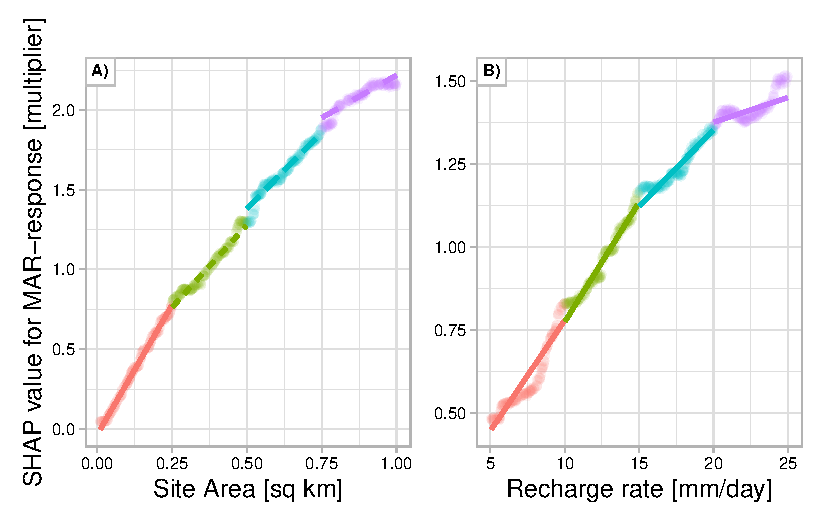
\includegraphics[keepaspectratio]{AqC6.3_paper2_V4_files/figure-pdf/fig-Analyze_site_area-1.pdf}}

}

\caption{\label{fig-Analyze_site_area}Decreasing effect of recharge
site) Trend in the SHAP values for the area of the recharge site and the
recharge rate at the site across their entire range. Four trend lines
are drawn through the points for each quantile to emphasize the changing
slope across the range.}

\end{figure}%

\subsection{Specific yield and groundwater
depth}\label{specific-yield-and-groundwater-depth}

\begin{figure}

\begin{minipage}{\linewidth}

\pandocbounded{\includegraphics[keepaspectratio]{D:/Dropbox/WUR/Rscripts/paper_2/depth_vs_rootzone_moisture.png}}

\end{minipage}%

\caption{\label{fig-depth_vs_rootzone}The relation between the moisture
content in the rootzone and the groundwater depth, as a scatter plot.
The moisture content is modeled by the unsaturated zone model MetaSWAP.
The moisture content is lower for locations with a deeper groundwater
which leads to a higher specific yield.}

\end{figure}%

\begin{figure}

\begin{minipage}{\linewidth}

\pandocbounded{\includegraphics[keepaspectratio]{D:/Dropbox/WUR/Rscripts/paper_2/depth_vs_sy.png}}

\end{minipage}%

\caption{\label{fig-depth_vs_sy}The relation between the specific yield
and the groundwater depth, as a scatter plot. The specific yield is
modeled by the unsaturated zone model MetaSWAP. The specific is lower
for locations with a deeper groundwater which leads to a higher specific
yield.}

\end{figure}%

\subsection{Specific yield and river
density}\label{specific-yield-and-river-density}

\begin{figure}

\begin{minipage}{\linewidth}

\pandocbounded{\includegraphics[keepaspectratio]{D:/Dropbox/WUR/Rscripts/paper_2/River_density_vs_rootzone_moisture.png}}

\end{minipage}%

\caption{\label{fig-river_density_vs_rootzone}The relation between the
moisture content in the rootzone and the river density, as a scatter
plot. The moisture content is modeled by the unsaturated zone model
MetaSWAP while the river density is calculated from the inputs to the
numerical groundwater model. The moisture content is lower for locations
with a deeper groundwater which leads to a higher specific yield.}

\end{figure}%

\begin{figure}

\begin{minipage}{\linewidth}

\pandocbounded{\includegraphics[keepaspectratio]{D:/Dropbox/WUR/Rscripts/paper_2/River_density_vs_Sy.png}}

\end{minipage}%

\caption{\label{fig-riv_vs_sy}The relation between the specific yield
and the river density, as a scatter plot. The specific yield is modeled
by the unsaturated zone model MetaSWAP while the river density is
calculated from the inputs to the numerical groundwater model. The
moisture content is lower for locations with a deeper groundwater which
leads to a higher specific yield.}

\end{figure}%




\end{document}
